
%page setup
\documentclass[12pt,twoside,a4paper,openright]{report}
%unicode encoding
\usepackage[utf8]{inputenc}

% Make latex understand and use the typographic
% rules of the language used in the document.
\usepackage[danish,english]{babel}
% Context Sensitive Quotation
\usepackage{csquotes}
% Use the palatino font
\usepackage[sc]{mathpazo}
\linespread{1.05}         % Palatino needs more leading (space between lines)

% Choose the font encoding
\usepackage[T1]{fontenc}
\usepackage{setspace} %Gives the possiblity to edit line spacing.
\usepackage[misc,clock,geometry]{ifsym}

% load a colour package
\usepackage{xcolor}
\definecolor{aaublue}{RGB}{33,26,82}% dark blue
% The standard graphics inclusion package
\usepackage{graphicx}
\usepackage{subfig}

% Set up how figure and table captions are displayed
\usepackage{float}

%%%%%%%%%%%%%%%%%%%%%%%%%%%%%%%%%%%%%%%%%%%%%%%%
% Mathematics
% http://en.wikibooks.org/wiki/LaTeX/Mathematics
%%%%%%%%%%%%%%%%%%%%%%%%%%%%%%%%%%%%%%%%%%%%%%%%
% Defines new environments such as equation,
% align and split 
\usepackage{amsmath}
\usepackage[makeroom]{cancel}
% Adds new math symbols
\usepackage{amssymb}
% Use theorems in your document
% The ntheorem package is also used for the example environment
% When using thmmarks, amsmath must be an option as well. Otherwise \eqref doesn't work anymore.
\usepackage[framed,amsmath,thmmarks]{ntheorem}

\usepackage{changepage}
% Change margins, papersize, etc of the document
\usepackage[
  showframe=false, %Shows margins on pages if necessary
  inner=25mm,% left margin on an odd page
  outer=25mm,% right margin on an odd page
  top=20mm,% Top margin on an odd page
  ]{geometry}
\usepackage{caption}
\captionsetup{%
  font=footnotesize,% set font size to footnotesize
  labelfont=bf % bold label (e.g., Figure 3.2) font
}

% Make the standard latex tables look so much better
\usepackage{array,booktabs}

% Enable the use of frames around, e.g., theorems
% The framed package is used in the example environment
\usepackage{framed}
\usepackage{wrapfig}
%\usepackage{background}
\usepackage{amsmath, amsfonts, amssymb}


%long tables enable page wide tables
\usepackage{longtable}
%array for aligning text in table
\usepackage{array}
%svg figures
\usepackage{svg}
\usepackage{tikz}
%\usepackage{ctable}



%%%%%%%%%%%%%%%%%%%%%%%%%%%%%%%%%%%%%%%%%%%%%%%%
% Mathematics
% http://en.wikibooks.org/wiki/LaTeX/Mathematics
%%%%%%%%%%%%%%%%%%%%%%%%%%%%%%%%%%%%%%%%%%%%%%%%
% Defines new environments such as equation,
% align and split 
\usepackage{amsmath}
\usepackage[makeroom]{cancel}
% Adds new math symbols
\usepackage{amssymb}
\usepackage{textcomp, gensymb}
% Use theorems in your document
% The ntheorem package is also used for the example environment
% When using thmmarks, amsmath must be an option as well. Otherwise \eqref doesn't work anymore.
\usepackage[framed,amsmath,thmmarks]{ntheorem}

\usepackage{changepage}
% Change margins, papersize, etc of the document
\usepackage[
  showframe=false, %Shows margins on pages if necessary
  inner=25mm,% left margin on an odd page
  outer=25mm,% right margin on an odd page
  top=20mm,% Top margin on an odd page
  ]{geometry}

  \usepackage{titlesec}
\titleformat{\chapter}[hang]{\normalfont\Huge\bfseries}{\thechapter: }{0pt}{\Huge}
\titleformat*{\section}{\normalfont\Large\bfseries}
\titleformat*{\subsection}{\normalfont\large\bfseries}
\titleformat*{\subsubsection}{\normalfont\normalsize\bfseries}
\titlespacing*{\chapter}{0pt}{-30pt}{40pt}
%\titleformat*{\paragraph}{\normalfont\normalsize\bfseries}
%\titleformat*{\subparagraph}{\normalfont\normalsize\bfseries}
\setlength{\parindent}{0pt}
\setlength{\headheight}{14.49998pt}
%afstand mellem kapitel og toppen af siden
\titlespacing*{\chapter}{0pt}{-40pt}{40pt}

% Clear empty pages between chapters
\let\origdoublepage\cleardoublepage
\newcommand{\clearemptydoublepage}{%
  \clearpage
  {\pagestyle{empty}\origdoublepage}%
}
\let\cleardoublepage\clearpage

% Change the headers and footers
\usepackage{fancyhdr}
\pagestyle{fancy}
\fancyhf{} %delete everything
\renewcommand{\headrulewidth}{0pt} %remove the horizontal line in the header
\fancyhead[RE]{\small\nouppercase\leftmark} %even page - chapter title
\fancyhead[LO]{\small\nouppercase\rightmark} %uneven page - section title
\fancyhead[LE,RO]{\thepage} %page number on all pages
% Do not stretch the content of a page. Instead,
% insert white space at the bottom of the page
\raggedbottom
% Enable arithmetics with length. Useful when
% typesetting the layout.
\usepackage{calc}
%setup of code snippets
\usepackage{listings}

\definecolor{gainsboro}{rgb}{0.86, 0.86, 0.86}
\definecolor{jokkesgraa}{rgb}{0.9490196078431372,0.9490196078431372,0.9215686274509803}
\lstdefinestyle{MatLab}{ %Formatting for code in appendix
    language=Matlab,
    numbers=left,
    frame=L,
    stepnumber=1,
    showstringspaces=false,
    tabsize=1,
    breaklines=true,
    breakatwhitespace=false,
    commentstyle=\itshape\color{green!40!black},
    keywordstyle=\bfseries\color{blue},
    backgroundcolor = \color{jokkesgraa},
}
\lstdefinestyle{C}{ %Formatting for code in appendix
    language=C, 
    numbers=left,
    frame=L,
    stepnumber=1,
    showstringspaces=false,
    tabsize=1,
    breaklines=true,
    breakatwhitespace=false,
    commentstyle=\itshape\color{green!40!black},
    keywordstyle=\color{blue},
    stringstyle=\color{orange!70!black},
    backgroundcolor = \color{jokkesgraa},
}
% Er lige ved at se om vi skal have en ekstra package for at definere farver
%prøv den her color code #f2f2eb alright alright
%%%%%%%%%%%%%%%%%%%%%%%%%%%%%%%%%%%%%%%%%%%%%%%%
% Bibliography
% http://en.wikibooks.org/wiki/LaTeX/Bibliography_Management
%%%%%%%%%%%%%%%%%%%%%%%%%%%%%%%%%%%%%%%%%%%%%%%%
\usepackage[nottoc]{tocbibind}
\usepackage[urldate=long,backend=biber,style=numeric,dateabbrev=false,sortcites,natbib=true,sorting=none]{biblatex}
\renewbibmacro*{urldate}{
(visited on \printfield{urlday}/\printfield{urlmonth}/\printfield{urlyear})
}
\addbibresource{bib/mybib.bib}%add bibliography as resource

%%%%%%%%%%%%%%%%%%%%%%%%%%%%%%%%%%%%%%%%%%%%%%%%
% Misc
%%%%%%%%%%%%%%%%%%%%%%%%%%%%%%%%%%%%%%%%%%%%%%%%
% Add bibliography and index to the table of
% contents
% Add the command \pageref{LastPage} which refers to the
% page number of the last page
\usepackage{lastpage}

% Add todo notes in the margin of the document
\usepackage[
  disable, %turn off todonotes
  colorinlistoftodos, %enable a coloured square in the list of todos
  textwidth=0.7\marginparwidth, %set the width of the todonotes
  textsize=scriptsize, %size of the text in the todonotes
  ]{todonotes}
\usepackage{parskip}
\setlength{\parskip}{1em}

\usepackage{hyperref}
\hypersetup{%
	plainpages=false,%
	pdfauthor={Gustav R T, Jakob T, Joachim A, Kasper Rødtnes, Thorvald Einarson},%
	pdftitle={AAU3, Reaction wheel stabilisation og inverse pendulum},%
	pdfsubject={Semester project},%
	bookmarksnumbered=true,%
	colorlinks=false,%
	citecolor=grey,%
	filecolor=black,%
	linkcolor=black,% you should probably change this to black before printing
	urlcolor=blue,%
	pdfstartview=FitH%
}
\usepackage{blindtext}
\usepackage{booktabs}
\usepackage{subcaption}
\usepackage{pdfpages}
\usepackage{colortbl}
\usepackage{booktabs,caption}
\usepackage[flushleft]{threeparttable}


\usepackage{titlesec}
\setcounter{secnumdepth}{4}

\titleformat{\paragraph}
{\normalfont\normalsize\bfseries}{\theparagraph}{1em}{}
\titlespacing*{\paragraph}
{0pt}{3.25ex plus 1ex minus .2ex}{1.5ex plus .2ex}

%Beautiful conditions
\usepackage{tabularx}
\newlength{\conditionwd}
\newenvironment{conditions}[1][where:]
  {%
   #1\tabularx{\textwidth-\widthof{#1}}[t]{
     >{$}l<{$} @{${}={}$} X@{}
   }%
  }
  {\endtabularx\\[\belowdisplayskip]}

%Beautiful conditions continiued
\newlength{\belongswd}
\newenvironment{belongs}[1][where:]
  {%
   #1\tabularx{\textwidth-\widthof{#1}}[t]{
     >{$}l<{$} @{${}\in {}$} X@{}
   }%
  }
  {\endtabularx\\[\belowdisplayskip]}

%\renewcommand*\contentsname{Summary} %Changes the name of the contents list
\usepackage[export]{adjustbox}
\usepackage{siunitx} % units
%\sisetup{}
%\sisetup{exponent-mode = engineering}
\sisetup{per-mode = symbol}
\usepackage{makecell}

\usepackage{subcaption}

\usepackage[super]{nth}% package inclusion and set up of the document
%  A simple AAU report template.
%  2015-05-08 v. 1.2.0
%  Copyright 2010-2015 by Jesper Kjær Nielsen <jkn@es.aau.dk>
%
%  This is free software: you can redistribute it and/or modify
%  it under the terms of the GNU General Public License as published by
%  the Free Software Foundation, either version 3 of the License, or
%  (at your option) any later version.
%
%  This is distributed in the hope that it will be useful,
%  but WITHOUT ANY WARRANTY; without even the implied warranty of
%  MERCHANTABILITY or FITNESS FOR A PARTICULAR PURPOSE.  See the
%  GNU General Public License for more details.
%
%  You can find the GNU General Public License at <http://www.gnu.org/licenses/>.
%
%
%
% see, e.g., http://en.wikibooks.org/wiki/LaTeX/Customizing_LaTeX#New_commands
% for more information on how to create macros

\newcommand{\e}{\mathrm{e}}
\newcommand{\mconst}[1]{\mathrm{#1}}

%%%%%%%%%%%%%%%%%%%%%%%%%%%%%%%%%%%%%%%%%%%%%%%%
% Macros for the titlepage
%%%%%%%%%%%%%%%%%%%%%%%%%%%%%%%%%%%%%%%%%%%%%%%%
%Creates the aau titlepage
\newcommand{\aautitlepage}[3]{%
  {
    %set up various length
    \ifx\titlepageleftcolumnwidth\undefined
      \newlength{\titlepageleftcolumnwidth}
      \newlength{\titlepagerightcolumnwidth}
    \fi
    \setlength{\titlepageleftcolumnwidth}{0.5\textwidth-\tabcolsep}
    \setlength{\titlepagerightcolumnwidth}{\textwidth-2\tabcolsep-\titlepageleftcolumnwidth}
    %create title page
    \thispagestyle{empty}
    \noindent%
    \begin{tabular}{@{}ll@{}}
      \parbox{\titlepageleftcolumnwidth}{
        \iflanguage{danish}{%
          
\includegraphics[width=\titlepageleftcolumnwidth]{aaugraphics/aau_logo_da.pdf}
        }{%
          
\includegraphics[width=\titlepageleftcolumnwidth]{aaugraphics/aau_logo_en.pdf}
        }
      } &
      \parbox{\titlepagerightcolumnwidth}{\raggedleft\sf\small
        #2
      }\bigskip\\
       #1 &
      \parbox[t]{\titlepagerightcolumnwidth}{%
      \textbf{Abstract:}\bigskip\par
        \fbox{\parbox{\titlepagerightcolumnwidth-2\fboxsep-2\fboxrule}{%
          #3
        }}
      }\\
    \end{tabular}
    \vfill
    \clearpage
  }
}

%Create english project info
\newcommand{\englishprojectinfo}[9]{%
  \parbox[t]{\titlepageleftcolumnwidth}{
    \textbf{Title:}\\ #1\bigskip\par
    \textbf{Theme:}\\ #2\bigskip\par
    \textbf{Project Period:}\\ #3\bigskip\par
    \textbf{Project Group:}\\ #4\bigskip\par
    \textbf{Participants:}\\ #5\bigskip\par
    \textbf{Supervisors:}\\ #6\bigskip\par
    \textbf{Copies:} #7\bigskip\par
    \textbf{Page Numbers:} #8 \\\bigskip\par
    \textbf{Date of Completion:}\\ #9
  }
}

%Create danish project info
\newcommand{\danishprojectinfo}[8]{%
  \parbox[t]{\titlepageleftcolumnwidth}{
    \textbf{Titel:}\\ #1\bigskip\par
    \textbf{Tema:}\\ #2\bigskip\par
    \textbf{Projektperiode:}\\ #3\bigskip\par
    \textbf{Projektgruppe:}\\ #4\bigskip\par
    \textbf{Deltager(e):}\\ #5\bigskip\par
    \textbf{Vejleder(e):}\\ #6\bigskip\par
    \textbf{Oplagstal:} #7\bigskip\par
    \textbf{Sidetal:} \pageref{LastPage}\bigskip\par
    \textbf{Afleveringsdato:}\\ #8
  }
}








%%%%%%%%%%%%%%%%%%%%%%%%%%%%%%%%%%%%%%%%%%%%%%%%
% An example environment
%%%%%%%%%%%%%%%%%%%%%%%%%%%%%%%%%%%%%%%%%%%%%%%%
\theoremheaderfont{\normalfont\bfseries}
\theorembodyfont{\normalfont}
\theoremstyle{break}
\def\theoremframecommand{{\color{gray!50}\vrule width 5pt \hspace{5pt}}}
\newshadedtheorem{exa}{Example}[chapter]
\newenvironment{example}[1]{%
		\begin{exa}[#1]
}{%
		\end{exa}
}
%%%%%%%%%%%%%%%%%%%%%%%%%%%%%%%%%%%%%%%%%%%%%%%%%%%%%%%%%%
%Macros
%%%%%%%%%%%%%%%%%%%%%%%%%%%%%%%%%%%%%%%%%%%%%%%%%%%%%%%%%%

\newcommand{\es}{\\[20pt]}

\newcommand{\subsubsubsection}[1]{
\paragraph{#1}
}

%Test command til at lave kommandoer med optional arguments.
%nr. 4 viser hvordan man kan lave en default hvis den er efterladt tom.
\newcommand{\test}[4][]{
\ifthenelse{\equal{#1}{}}{}{#1 \\[20pt]}
\ifthenelse{\equal{#2}{}}{}{#2 \\[20pt]}
\ifthenelse{\equal{#3}{}}{}{#3 \\[20pt]}
\ifthenelse{\equal{#4}{}}{default value}{#4}
}

\newcommand{\AAU}[1][]{AAU$^3$ }

\DeclareSIUnit{\kmph}{\kilo \meter\per\hour}

%\test[XXX]{AAA}{BBB}{CCC}
%Til PDF i appendix
\newcommand{\pdfappendix}[3][]{
\includepdf[pages=1,scale=1,pagecommand={\subsection{#1}\label{#2}},linktodoc=true]{#3}
\includepdf[pages=2-,scale=1,linktodoc=true]{#3}
}
%Til Chapter
\newcommand{\Chap}[2]{\chapter{#1}\label{ch:#2}}

%Dette gøres ved at skrive \Chap{}{}, hvor den første er Titlen og den anden er label.
%Til Section
\newcommand{\Sec}[2]{\section{#1}\label{sec:#2}}

%Til SubSection
\newcommand{\Sub}[2]{\subsection{#1}\label{subsec:#2}}

%Til SubsubSection
\newcommand{\Subsub}[2]{\subsubsection{#1}\label{subsubsec:#2}}
%%%%%%%%%%%%%%%%%%%%%%%%%%%%%%%%%%%%%%%%%%%%%%%%











% my new macros


% \begin{document}
\begin{document}

\raggedright
 \pdfbookmark[0]{Frontpage}{label:frontpage}%

 \begin{titlepage}
 %background waves
     \tikz[remember picture,overlay]
     \node[opacity=1,inner sep=0pt]
     at (current page.center)
     {
\includegraphics[width=\paperwidth,height=\paperheight]{aaugraphics/aau_waves.pdf}};
 %background waves end 

  \fboxsep0pt\colorbox{aaublue}

   \vfill% add spacing 
    \noindent

    {\colorbox{aaublue}{\begin{tabular}{@{}p{\textwidth}@{}}% Adding box
    \color{white}
     \begin{center}
     \Huge{\textbf{Characterizing passive components}}
     \end{center}
     \vspace{0.2cm}
    \begin{center}
     {\Large
        Joachim R.B. Andersen\\
        Jakob F. Thiesen\\
      }
     \vspace{0.4cm}
     {\large
       Bachelor of Engineering of Electronics, 7th semester, 2024
     }
    \end{center}
    \vspace{0.2cm}
   \end{tabular}}}
 
   \vfill %spacing
   \begin{center} %add circle logo
     
\includegraphics[width=0.2\paperwidth]{aaugraphics/aau_logo_circle_en.pdf}
   \end{center}
 \end{titlepage}
 \clearpage

\selectlanguage{english}
\pdfbookmark[0]{Danish title page}{label:titlepage_en}

\aautitlepage{%
  \englishprojectinfo{
     %title
     Design of a Spectral Impedance Analyzer for Passive Elements
  }{%
    Designing and constructing an Impedance Analyzer%theme
  }{%
    Fall Semester 2024 %project period
  }{%
    Group 771 - EIT7% project group
  }{%
    %list of group members
    Joachim R.B. Andersen\\
    Jakob F. Thiesen
    
  }{%
    %list of supervisors
    %The omnissiah
    Troels B. Sørensen
  }{%
    2 % number of printed copies
  }
  { %number of pages in the main matter
   A lot
  }
  {%
    \today % date of completion
  }%
}{%department and address
  \textbf{Electronics and IT}\\
  Aalborg University\\
  \href{http://www.aau.dk}{http://www.aau.dk}
}{% the abstract
This project focused on the development of a cost-effective impedance analyzer specifically designed for the characterization of passive components such as capacitors and inductors.

The initial phase involved a problem analysis to identify the target market, assess existing impedance analyzers in terms of functionality, cost, and accessibility. Our analysis revealed a gap in the market for a device that combines key features of high-end instruments at a price point accessible to a broader audience, including hobbyists, educational institutions, and small-scale enterprises.

Based on this, we developed an impedance analyzer with specifications aimed at delivering high performance at a reduced cost. The design phase included defining critical system requirements, followed by a lengthy hardware, and software, design phase and culminating in the creation of a PCB. The PCB was subsequently tested to validate the projects functionality against the set specifications.

The resulting impedance analyzer demonstrated capabilities for measuring impedance across a wide frequency range and is suitable for characterizing important parameters of passive components. This project offers a practical solution for affordable impedance measurement but also contributes to making advanced electronic testing equipment more accessible to the general public.
}

\thispagestyle{empty}
\chapter*{Preface}\label{ch:preface}

This report was written during the 7th semester of the Bachelor of Engineering of Electronics at Aalborg University in the 2024 fall semester and documents the work being done as part of the bachelors project.

The topic of this project is to analyze what an impedance analyzer is, how it works, why it is expensive and if it is possible to design and construct a cheaper, but still capable, instrument to do the same job as the commercially available instruments.

This report is confidential and the authors request that this document not be shared or distributed in any way without permission from the authors.

\vspace{\baselineskip}\hfill Aalborg University, \today


\begin{minipage}[b]{0.45\textwidth}
 \centering
 {\setstretch{0.1}
 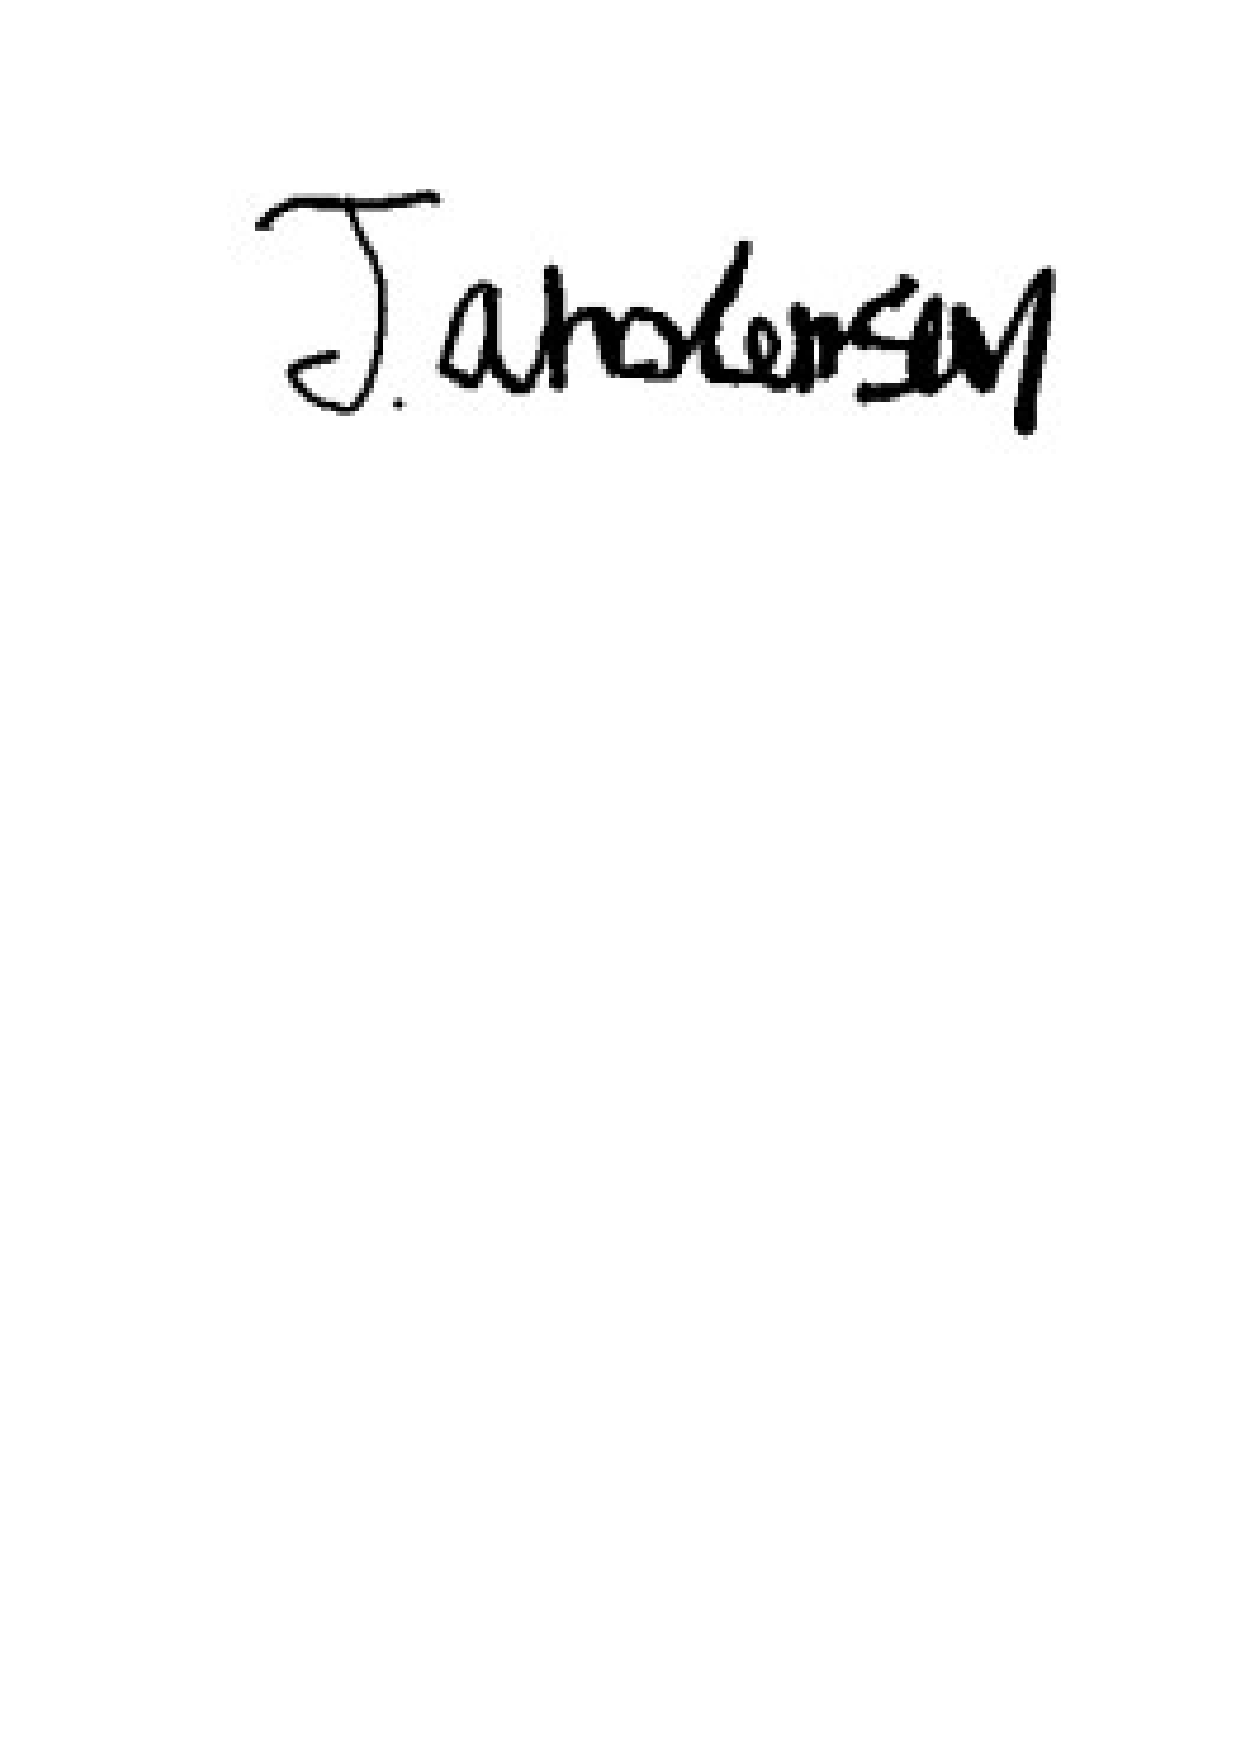
\includegraphics[clip, trim=0 600 0 0, width=0.8\textwidth]{Formalia/Figures/Jsig.pdf}
 \rule{\textwidth}{0.5pt}\\}
 Joachim R.B. Andersen\\
 {\footnotesize <jander20@student.aau.dk>}
 {\footnotesize <j.rixen@outlook.dk>}
\end{minipage}
\hfill
\vspace{5pt}
\begin{minipage}[b]{0.45\textwidth}
 \centering
 {\setstretch{0.1}
 
\includegraphics[clip, trim=0 575 0 0, width=0.8\textwidth]{Formalia/Figures/JakSig.pdf}
 \rule{\textwidth}{0.5pt}\\}
 Jakob F. Thiesen\\
 {\footnotesize <jfth21@student.aau.dk>}
 {\footnotesize <jakob.thiesen97@gmail.com>}
\end{minipage}


\tableofcontents
\clearpage
%


\section{References, labels and abbreviations}
% Please add the following required packages to your document preamble:
% \usepackage[table,xcdraw]{xcolor}
% If you use beamer only pass "xcolor=table" option, i.e. \documentclass[xcolor=table]{beamer}
\begin{table}[H]
\begin{tabular}{|l|l|}
\hline

Section type  & Reference/Label name \\ \hline
Chapter       & ch:name                  \\ \hline
Section       & sec:name                  \\ \hline
Subsection    & subsec:name               \\ \hline
Subsubsection & subsubsec:name           \\ \hline
Figure        & fig:name                  \\ \hline
Table         & tab:name                  \\ \hline
Equation      & eq:name                   \\ \hline
code snippets & snip:name                 \\ \hline
Appendix      & app:name                  \\ \hline
Bibliography  & bib:name\_addition\_another\_addition                \\ \hline
\end{tabular}
\end{table}
\section{Figures and tables}
\subsection{2 by x table}
\begin{table}[H]
\begin{tabular}{|l|l|}
\hline

        &       \\ \hline
        &       \\ \hline
        &       \\ \hline
\end{tabular}
\end{table}

\subsection{3 by x table}
\begin{table}[H]
\begin{tabular}{|l|l|l|}
\hline

        &       &       \\ \hline
        &       &       \\ \hline
        &       &       \\ \hline
\end{tabular}
\end{table}
\subsection{colored 3 by x table}
\begin{table}[H]
\begin{tabular}{|l|l|l|}
\hline
 
&  &  \\ \hline
 &  &  \\ \hline
 &  &  \\ \hline
\end{tabular}
\end{table}

\subsection{Figure figure}
Inserting figures of type: PDF, JPEG, JPG, PNG
\begin{figure}[H]
    \centering
    
\includegraphics[width=0.5\textwidth]{aaugraphics/aau_logo_circle_en.pdf}
    \caption{Caption}
    \label{fig:enter_label2}
\end{figure}

\subsection{SVG figure}
\begin{figure}[H]
    \centering
    \includesvg[width=0.3\textwidth]{Sections/1_Introduction/figures/Smiley.svg}
    \caption{ SVG smiley. He is happy be cause the file size is small but the resolution is high}
    \label{fig:enter_label1}
\end{figure}

\section{Unit and equations}
Examples of how to use units and different equations
\subsection{SI units}

\subsection{Equations}
\paragraph*{numerated equation:}
In equation \ref{ex:eq1} how to set up a enumerated equation can be seen.
\begin{equation}\label{ex:eq1}
    K_T = \frac{\tau}{I_a}
\end{equation}
\begin{conditions}
    K_T     & motor constant\\
    \tau    & the torque the motor produces\\
    I_a     & the current the motor draws\\
\end{conditions}


\paragraph*{unnumerated equation:}
In equation \ref{ex:eq2} how to set up an unenumerated equation can be seen. The reference however is changed to the nearest reference-able title object. Always try to add a reference to the equation, it might come in handy.
\begin{equation*}\label{ex:eq2}
    K_T = \frac{\tau}{I_a}
\end{equation*}
\begin{conditions}
    K_T     & motor constant\\
    \tau    & the torque the motor produces\\
    I_a     & the current the motor draws\\
\end{conditions}

\paragraph*{How to do math in latex}
If the table below is not fulfilling:
\url{https://www.cmor-faculty.rice.edu/~heinken/latex/symbols.pdf}

\begin{table}[H]
\centering
\renewcommand{\arraystretch}{1.5}
\begin{tabular}{|l |c|l|} \hline   
addition & + & + \\ \hline 
subtraction & - & - \\ \hline 
multiplication & $\cdot$ & \textbackslash{cdot} \\ \hline 
division & $\frac{num}{denom}$ & \textbackslash{frac\{num\}\{denom\}} \\ \hline 
powers & $a^{b+c}$ & a\^ \space\{b+c\}\\ \hline 
square root & $\sqrt{a+b} $ & \textbackslash{sqrt(a+b)} \\ \hline 
summation & $\sum $ & \textbackslash{sum} \\ \hline 
integration & $\int$ & \textbackslash{}int \\ \hline 
2x int & $\iint$ & \textbackslash{}iint \\ \hline 
3x int & $\iiint$ & \textbackslash{}iiint \\ \hline 
differentiation & $\dot{a}$ & \textbackslash{Ddot\{a\{}\\ \hline 
2x diff & $\Ddot{a}$ & \textbackslash{Ddot\{a\{}\\ \hline 
vector notation & $\overline{\rm AB}$  & \textbackslash{}overline\{\rm AB\}  \\ \hline

\end{tabular}

\end{table}




% Introduction
\chapter{Introduction} \label{ch:Introduction}
Among hobbyists, tinkerers and smaller companies, there is a need to characterize the most basic one-port electronic devices such as capacitors, inductors and resistors. Resistors can be bought, relatively, cheaply while still having a high degree of accuracy. Inductors and capacitors, however, often have significantly looser tolerances. Another limitation of reactive devices is the level of detail provided in their datasheets. Often values such as ESR or phase angle are not stated, nor their frequency or bias voltage stability. These parameters can be crucial for a designer when engineering an accurate, reliable and predicable circuit.

These component parameters can be measured, or at least somewhat estimated by the means of a rather large and complicated test-setup, involving both signal generators and oscilloscopes. The amount of steps required to take measurements such as these makes it prone to human errors and errors inherent to the test setup. As an added constraint; the test procedure is tedious to perform and, because of the limited range of the setup, the results can be inaccurate, especially at higher frequencies.

Professional test equipment for exactly this purpose is available on the market and are known in the industry as LCR meters. These devices come in a broad range of measurement capabilities and frequency ranges. Whilst these devices are available, the LCR meters with both good accuracy, flexible capabilities and high frequency ranges are prohibitively expensive and beyond the reach of most individuals, and small companies. These issues leads to the initial problem statement of this project.

“Why are these high-end LCR meters so expensive? Is it possible to estimate the characteristics of a passive device in a more economical way than what is present on the market today?”


% Problem Analyse
\chapter{Problem Analysis} \label{ch:ProblemAnalysis}
This section seeks to explain how passive components can, generally, be characterized and what instruments are commercially available to do it. The section will also discuss which requirements both professional and individuals may have for an LCR meter and what a reasonable price point may be for an individual.
\section{Measuring reactive components} \label{sec:MeasureReactiveComponents}

testfafafa
\section{Commercial Instruments} \label{sec:CommercialImpedanceMeasurement}
Most of the major manufacturers of test equipment, such as Keysight Technologies, Rohde \& Schwarz, Tektronix and others produce a range of instruments for characterizing passive components. This section will sample a few of these to research their capabilities, to indicate what a user might want and need. The instruments are chosen based on their perceived price range. 

LCR meters typically come in two different form factors, one is a handheld device, much like a regular multimeter, while the other is a benchtop instrument. The handheld LCR meters, like the Keysight U1733C\cite{KeysightU1733C}, shown in figure \ref{fig:2_2_U1733C}.
\begin{figure}[H]
    \centering
    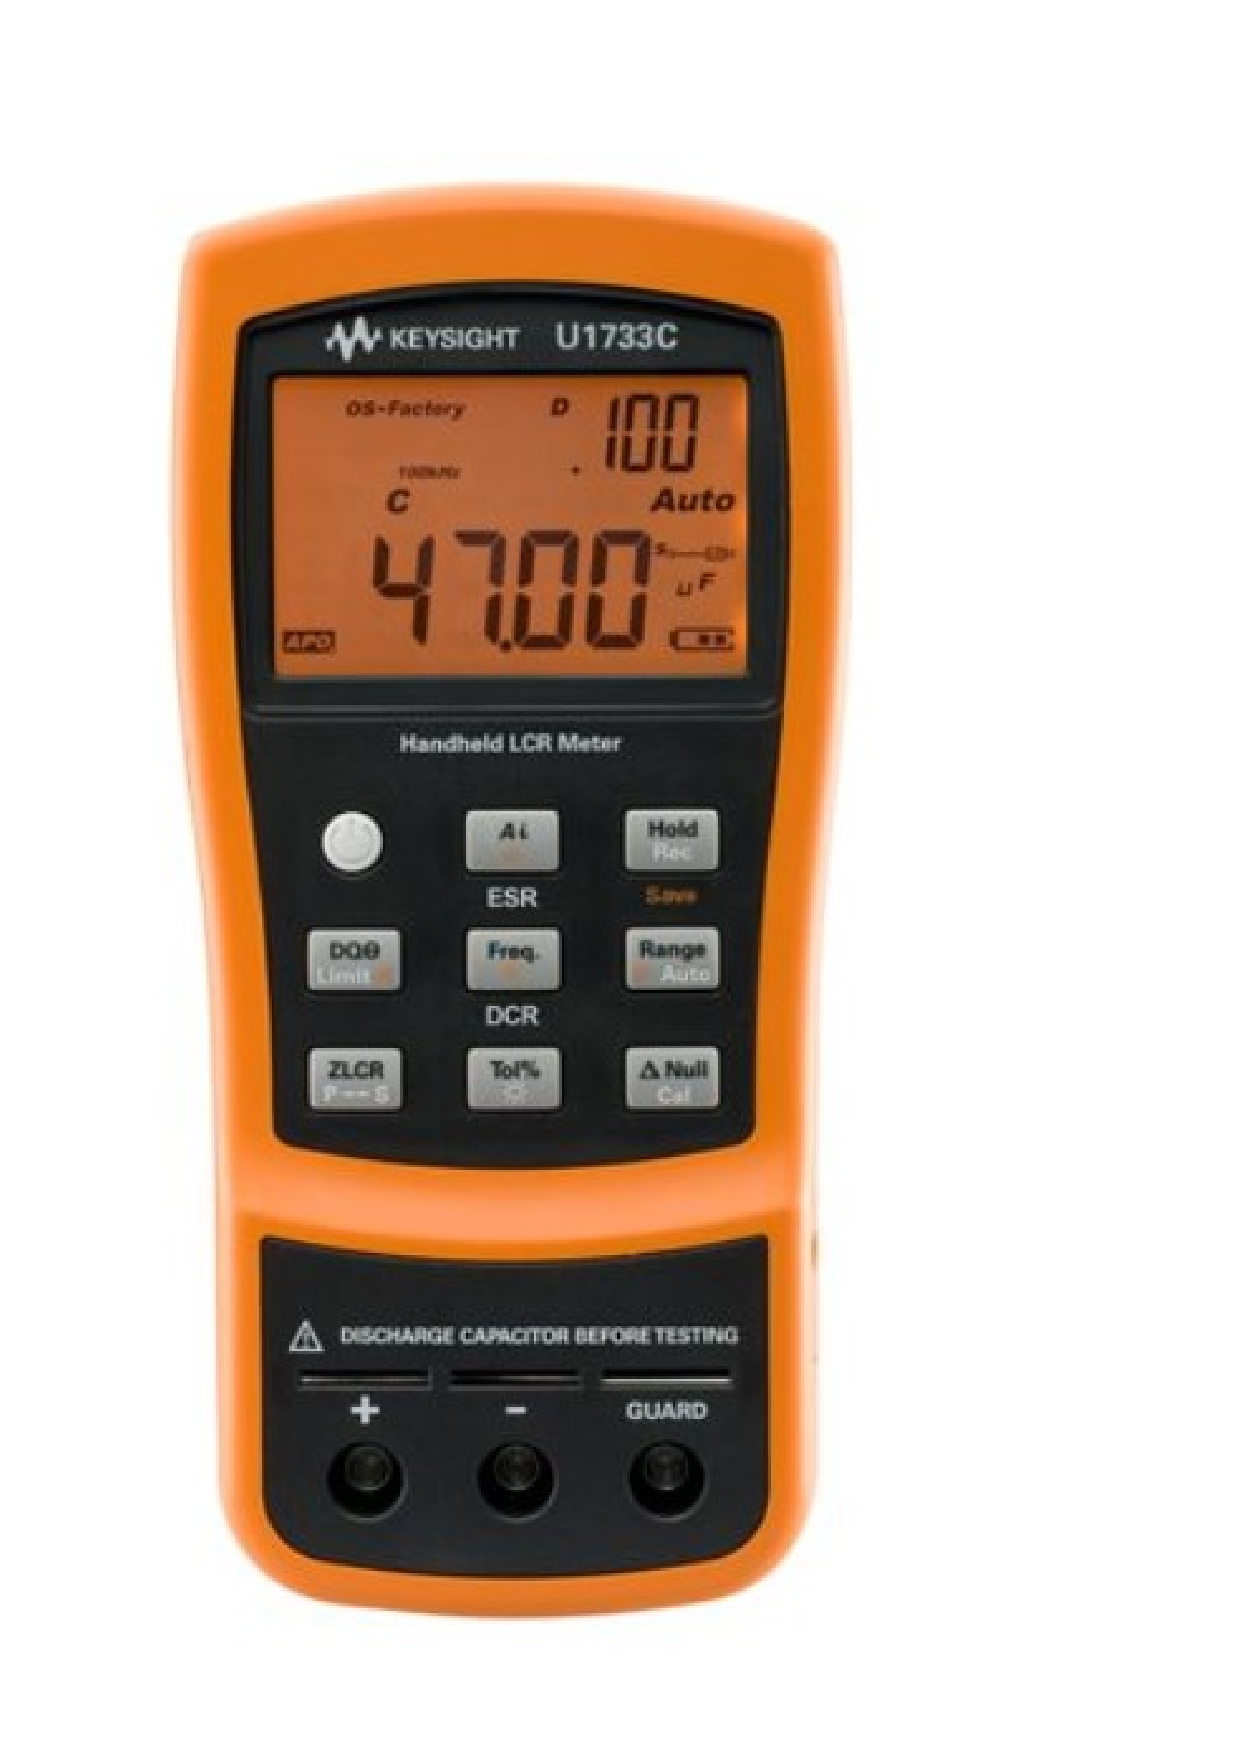
\includegraphics[clip, trim=0 50 0 50, width=0.5\textwidth]{Sections/2_ProblemAnalysis/FIgures/KeysightU1733C.pdf}
    \caption{A handheld Keysight U1733C LCR meter.\cite{KeysightU1733C}}
    \label{fig:2_2_U1733C}
\end{figure}
The U1733C shown on \ref{fig:2_2_U1733C} is meant for, primarily, troubleshooting and repair work and not electronics development purposes, while it is affordable at about 550€, it has limited capabilities. It can measure all the basic parameters such as capacitance, inductance, ESR and display all the derived quantities like dissipation and quality factor, see section \refq{subsec:DerivedQuantities} for further explanation. Numerically, however it can only take these measurements at a pre-determined set of test frequencies in the range \SI[]{100}{\hertz} to \SI[]{100}{\kilo\hertz} with measurement accuracy weaning off in both ends of the impedance range, and at higher frequencies.

Table \refq{tab:2_3_AccuracyTab_U1733C} shows the accuracy the impedance magnitude for the U1733C at the high and low end of the impedance ranges, as well as over a range of frequencies. Table \refq{tab:2_3_PhaseAccuracyTab_U1733C} shows the corresponding phase angle accuracy at the same impedances and frequencies. It clearly shows that at the extremes of impedance the accuracy degrades.

\begin{table}[H]
  \begin{tabular}{|m{6.3em}|m{6.3em}|m{6.3em}|m{6.3em}|m{6.3em}|}
  \hline
   Frequency / \nl Applied \nl Impedance & \SIQ{100}{\hertz} & \SIQ{1}{\kilo\hertz} & \SIQ{10}{\kilo\hertz} & \SIQ{100}{\kilo\hertz} \\ \hline
  \SIQ{1}{\ohm}    &   \SIQ{1.2}{\%}   &   \SIQ{1.2}{\%}    &   \SIQ{1.2}{\%}     &   \SIQ{1.5}{\%}      \\ \hline
  \SIQ{10}{\ohm}   &   \SIQ{0.78}{\%}     &  \SIQ{0.78}{\%} & \SIQ{0.78}{\%}  & \SIQ{0.78}{\%}    \\ \hline
  \SIQ{1}{\kilo\ohm}   &   \SIQ{0.23}{\%}     & \SIQ{0.23}{\%}  &  \SIQ{0.23}{\%}  & \SIQ{0.55}{\%} \\ \hline
  \SIQ{100}{\kilo\ohm} &   \SIQ{0.55}{\%}     &  \SIQ{0.55}{\%}  & \SIQ{0.55}{\%}   & \SIQ{0.78}{\%}  \\ \hline
  \SIQ{100}{\mega\ohm} &   \SIQ{6.8}{\%}     &   \SIQ{6.8}{\%}  &  NA   &   NA  \\ \hline
  \end{tabular}
  \caption{Table of selected impedance measurement accuracy of a U1733C. It can be seen that the accuracy degrades at higher frequencies and at the extreme ends of the impedance capabilities.}
  \label{tab:2_3_AccuracyTab_U1733C}
  \end{table}


  \begin{table}[H]
    \begin{tabular}{|m{6.3em}|m{6.3em}|m{6.3em}|m{6.3em}|m{6.3em}|}
    \hline
     Frequency / \nl Applied \nl Impedance & \SIQ{100}{\hertz} & \SIQ{1}{\kilo\hertz} & \SIQ{10}{\kilo\hertz} & \SIQ{100}{\kilo\hertz} \\ \hline
    \SIQ{1}{\ohm}    &   \SIQ{0.69}{\degree} &   \SIQ{0.69}{\degree} &   \SIQ{0.69}{\degree}  &  \SIQ{0.86}{\degree}  \\ \hline
    \SIQ{10}{\ohm}   &   \SIQ{0.45}{\degree}     &  \SIQ{0.45}{\degree} & \SIQ{0.45}{\degree}  & \SIQ{0.45}{\degree}  \\ \hline
    \SIQ{1}{\kilo\ohm}   &  \SIQ{0.13}{\degree}  & \SIQ{0.13}{\degree}  &  \SIQ{0.13}{\degree}  & \SIQ{0.32}{\degree} \\ \hline
    \SIQ{100}{\kilo\ohm} &   \SIQ{0.32}{\degree} &  \SIQ{0.32}{\degree} & \SIQ{0.32}{\degree}  & \SIQ{0.45}{\degree}  \\ \hline
    \SIQ{100}{\mega\ohm} &   \SIQ{3.90}{\degree}     &   \SIQ{3.90}{\degree}  &  NA   &   NA  \\ \hline
    \end{tabular}
    \caption{Table of selected phase angle measurement accuracy of a U1733C. It can be seen that the accuracy degrades at higher frequencies and at the extreme ends of the impedance capabilities.}
    \label{tab:2_3_PhaseAccuracyTab_U1733C}
    \end{table}


The U1733C datasheet has similar charts for other measurements, but they follow a similar pattern of accuracy as capacitance where it becomes clear that the accuracy is worse in the higher ends of the range. The accuracy is listed as a $\%$ of range $ + n\cdot resolution$, so a measurement in the \SI[]{20}{\micro\farad} range will have an accuracy of $\pm \SI[]{1}{\micro\farad} + \SI[]{10}{\nano\farad} = \SIQ{1.01}{\micro\farad}$ at \SIQ{100}{\kilo\hertz}.

Rohde \& Schwarz has a benchtop line of LCR meters called the LCX line \cite{RSLCXLCRMeters}. These have tighter specifications for accuracy, a greater range and a more diverse set of displaying the measurements. They also come with a significantly higher price tag at 15000€ for a 500kHz bandwidth version. This LCR meter is shown on figure \ref{fig:2_2_RSLCX}.
\begin{figure}[H]
    \centering
    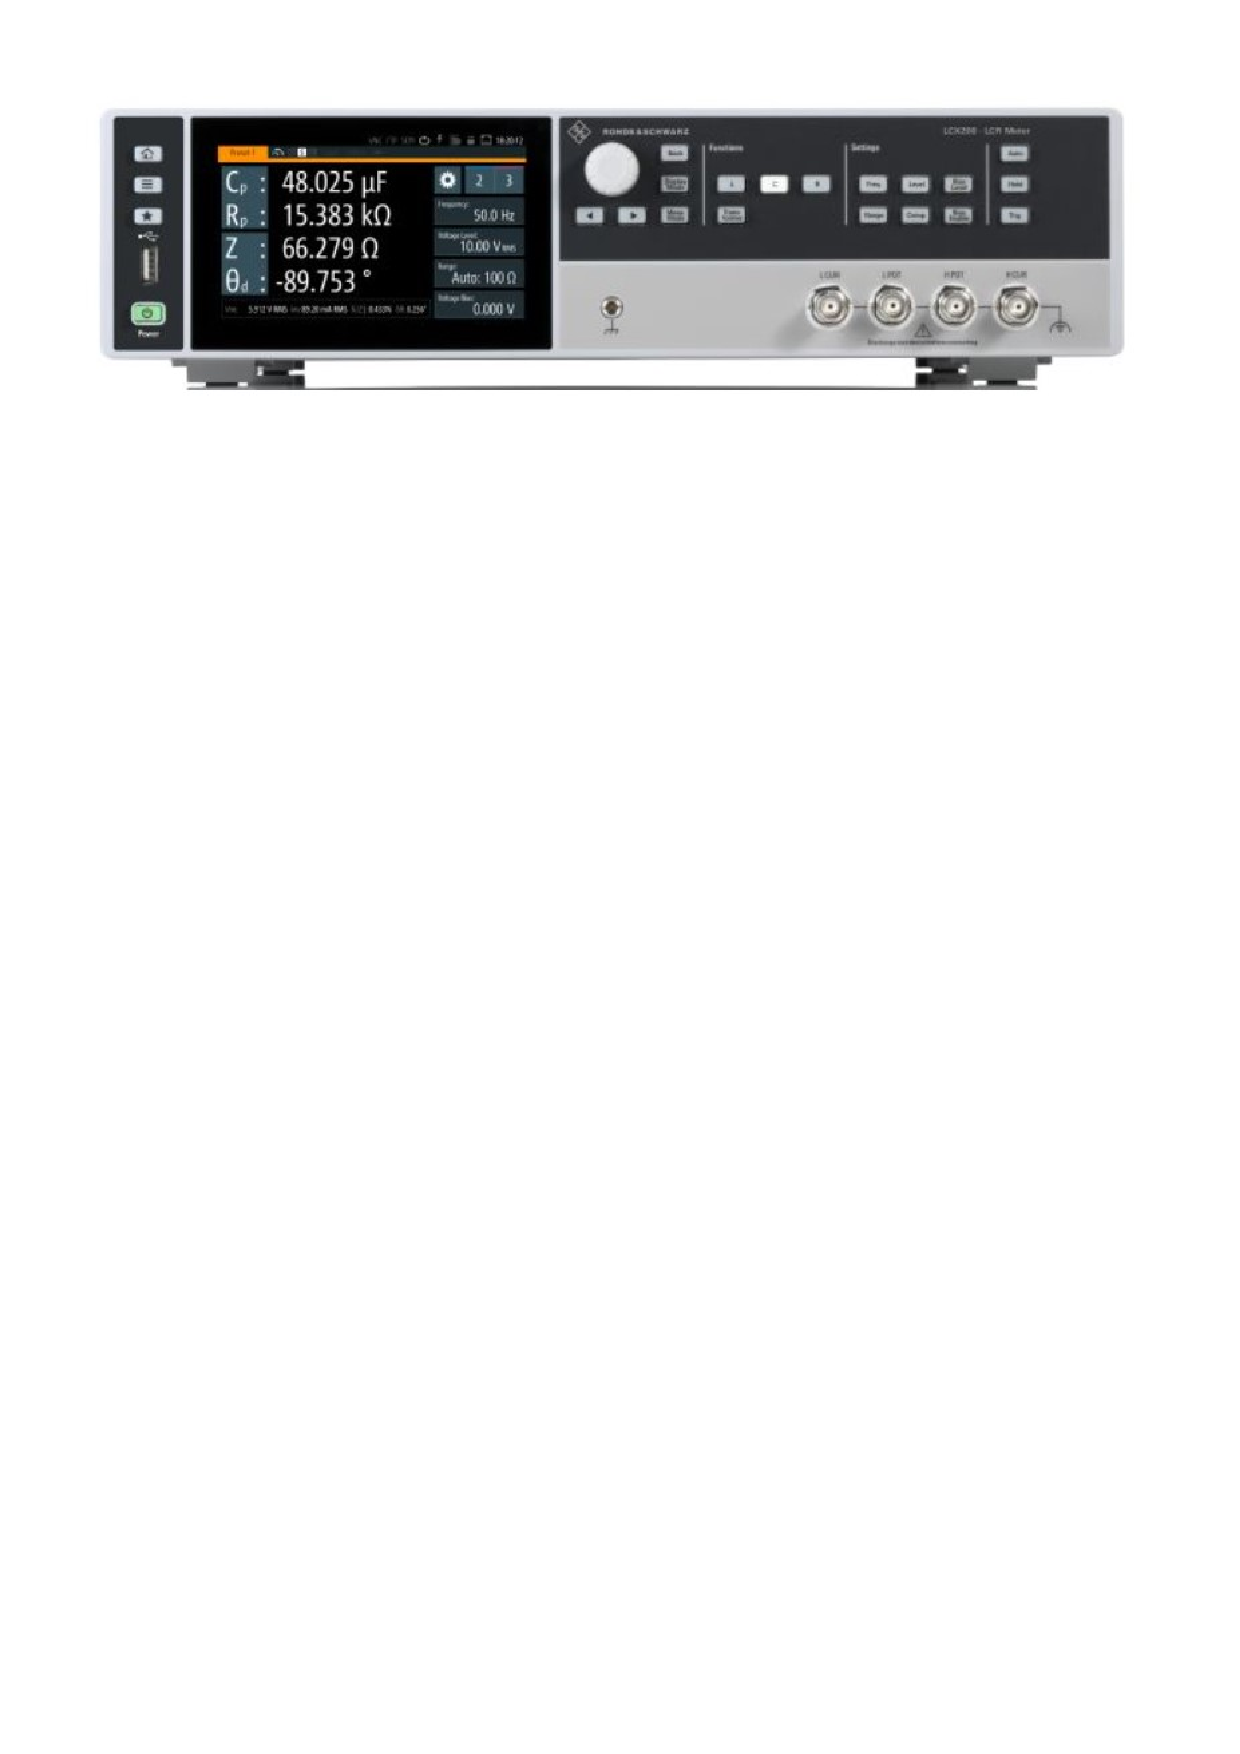
\includegraphics[clip, trim=0 630 0 50, width=1\textwidth]{Sections/2_ProblemAnalysis/FIgures/RSLCXLCR.pdf}
    \caption{A Rohde \& Schwarz LCX LCR meter featured a significantly greater bandwidth when compared to the U1733C, 4-wire kelvin measurements and greater ability to display the measurements.\cite{RSLCXLCRMeters}}
    \label{fig:2_2_RSLCX}
\end{figure}

The Rohde \& Schwarz LCX LCR meter is using kelvin bridge (4-wire) measurements.  This feature is often seen on higher end test equipment in order for the instrument to compensate for the parasitics introduced by the test instruments own test leads. The instrument can be triggered to take measurements externally and be controlled remotely over various network interfaces. The meter also has a sweep function in order to measure the impedance of the DUT over a series of frequency values and can display all the measurements numerically of graphically. Unlike the U1733C this meter is intended for electronic development purposes.

The Wayne-Kerr 6500B\cite{WayneKerr6500} series is a high-end impedance analyzer for demanding applications. The industry differentiates between \textit{LCR meters} and \textit{Impedance analyzers}. An LCR meter will display it's single point measurements numerically, while an impedance analyzer can do the same but is meant specifically for frequency sweeps and displaying the measurements on graphs. In other words, an impedance analyzer is a more advanced LCR meter. The Wayne-Kerr 6500B is shown on figure \ref{fig:2_2_WayneKerr6500B}. 
\begin{figure}[H]
    \centering
    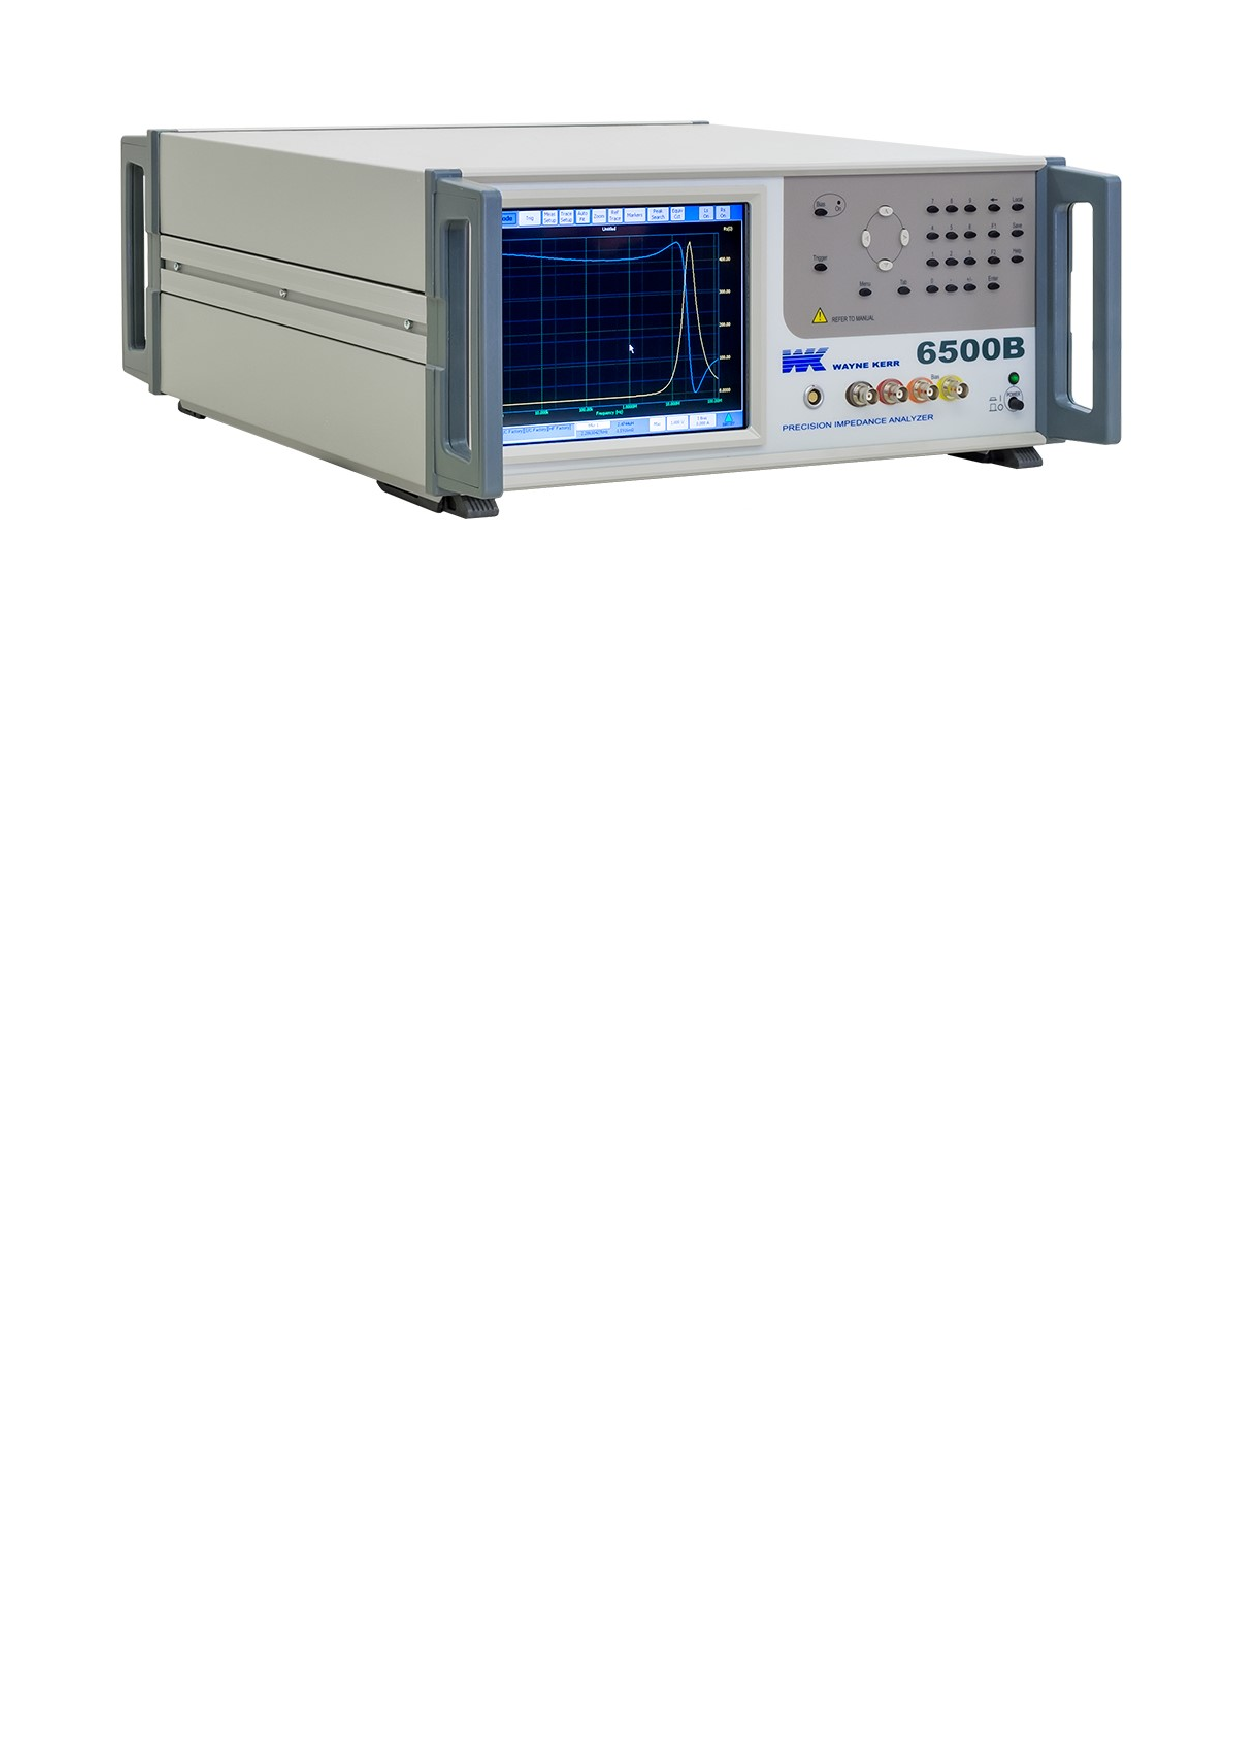
\includegraphics[clip, trim=0 550 0 50, width=1\textwidth]{Sections/2_ProblemAnalysis/FIgures/WayneKerrImpedanceAnalyzer.pdf}
    \caption{A Wayne-Kerr 6500B impedance analyzer. Note how it displays it's measurements graphically.}
    \label{fig:2_2_WayneKerr6500B}
\end{figure}
This impedance analyzer has a test frequency range of \SI[]{20}{\hertz} to \SI[]{120}{\mega\hertz} and has a test frequency resolution of \SI[]{100}{\micro\hertz} and Wayne-Kerr guarantees an accuracy of L, C and R measurements of $\pm 0.05$ \% across the entire frequency range putting this instrument in a different league from the ones previously shown. This impedance analyzer has adjustable DC bias as well, so bias stability can be measured as well. The impedance analyzer can display it's measurements on regular plots but can also show them in polar, or complex, form much like a network analyzer. The price of this instrument is listed as \textit{request quote} putting it far out of reach of even most smaller companies.

A few LCR meters and impedance analyzers were reviewed, there are many more but it would be impractical to list all of them. It was done in order to analyze what functionality they have. Their functionality and price points are closely related and a table has been made to break down the overall capabilities of each instrument. The results for this can be seen in table \ref{tab:2_3_CapabilityTab}.

\begin{table}[H]
  \begin{tabular}{|m{9.5em}|m{8em}|m{8em}|m{8em}|}
  \hline
    &   Keysight U1733C       & Rohde \&\newline Schwartz LCX      & Wayne-Kerr\newline 6500B                 \\ \hline
    Test frequency range      &  \SI[]{20}{\hertz} to \SI[]{100}{\kilo\hertz}$\mathbf{^1}$     &    DC-\SI[]{500}{\kilo\hertz},\newline \SI[]{1}{\hertz} steps   & \SI[]{20}{\hertz}-\SI[]{120}{\mega\hertz},\newline  \SI[]{100}{\micro\hertz} steps                                                  \\ \hline
    Basic accuracy$\mathbf{^2}$            &  [Z] 0.2\%\newline [$\phi$] $0.2$\%      & [Z] $\pm 0.05$\%\newline [$\phi$] $\pm 0.03$\degree       &[Z] $\pm 0.05$\%\newline [$\phi$] $\pm 0.0005$\degree                                                    \\ \hline
    Interface Type            &  Simple$\mathbf{^3}$\nl LCD, buttons    & Touchscreen & Touchscreen \\ \hline
    Measurement mode          &   2-wire    & 4-wire      & 4-wire                                  \\ \hline
    Auto ranging              &   Yes    & Yes      & Yes                                           \\ \hline
    Adj. DC Bias range        &   No    & \SIQ{40}{\volt}DC$\mathbf{^4}$      & $\pm$\SIQ{40}{\volt}DC           \\ \hline
    Frequency sweep           &   No    & Yes$\mathbf{^5}$      & Yes                               \\ \hline
    Data logging              &   No    & Yes      & Yes                                            \\ \hline
    Component binning         &   No    & Yes      & Yes                                            \\ \hline
    Graph data point          &   No    & Yes      & Yes                                            \\ \hline
    Complex plane plots       &   No    & No       & Yes                                             \\ \hline
    Network access            &   No    & Yes      & Yes                                  \\ \hline
    Price point               & <1000€   & 15000€   & Undisclosed                                    \\ \hline
  \end{tabular}
  \caption*{
    \raggedright
    $\mathbf{^1}$ The test frequencies for the U1733C are in pre-determined steps.\\
    $\mathbf{^2}$ \textit{Z} refers to impedance measurement accuracy. \textit{$\phi$} refers specifically to the phase measurement. The term \textit{basic accuracy} covers the minimum accuracy of L, C, R, ESR, D, Q measurements across the frequency range of the instrument.\\
    $\mathbf{^3}$ \textit{simple} refers to the instruments U/I being a few buttons and an LCD display as shown on figure \ref{fig:2_2_U1733C}.\\
    $\mathbf{^4}$ The Rohde \& Schwartz LCX DC bias setting is an extra software options that can be purchased\\
    $\mathbf{^5}$ The Rohde \& Schwartz LCX can do frequency sweeps if an extra software option is purchased.\\
  }
  \caption{A summary of the capabilties of the 3 instruments.}
  \label{tab:2_3_CapabilityTab}
\end{table}

As shown in table \ref{tab:2_3_CapabilityTab} there is a clear distinction in the level of features available at different price points and the major differentiator in their price is the instruments accuracy and test frequency range. The U1733C is affordable for most individuals but lacks a lot of the functions and range available at higher price brackets. The LCX and 6500B will have significantly more advanced hardware and a major difference between these two is there test frequency ranges. It is noteworthy how some of their features are due to them having more advanced software and interfaces. Some of these features could be made available in a lower price bracket with software alone. 



\section{Commercial Instruments Capabilities} \label{sec:CommercialImpedanceAnalyzerCapabilities}
A few LCR meters and impedance analyzers were reviewed in section \ref{sec:CommercialImpedanceMeasurement}, there are many more but it would be impractical to list all of them, it was done in order to analyze what functionality they have. Their functionality and price points are, however, closely related. This section seeks to break down some of the functionality a customer could expect at certain price points. The results for this can be seen in table \ref{tab:2_3_CapabilityTab}.

\begin{table}[H]
  \begin{tabular}{|m{9.5em}|m{8em}|m{8em}|m{8em}|}
  \hline
    &   Keysight U1733C       & Rohde \&\newline Schwartz LCX      & Wayne-Kerr\newline 6500B                 \\ \hline
    Test frequency range      &  \SI[]{20}{\hertz} to \SI[]{100}{\kilo\hertz}$\mathbf{^1}$     &    DC-\SI[]{500}{\kilo\hertz},\newline \SI[]{1}{\hertz} steps   & \SI[]{20}{\hertz}-\SI[]{120}{\mega\hertz},\newline  \SI[]{100}{\micro\hertz} steps                                                  \\ \hline
    Basic accuracy$\mathbf{^2}$            &  [Z] 0.2\%\newline [$\phi$] $0.2$\%      & [Z] $\pm 0.05$\%\newline [$\phi$] $\pm 0.03$\degree       &[Z] $\pm 0.05$\%\newline [$\phi$] $\pm 0.0005$\degree                                                    \\ \hline
    Interface Type            &  Simple$\mathbf{^3}$\nl LCD, buttons    & Touchscreen & Touchscreen \\ \hline
    Measurement mode          &   2-wire    & 4-wire      & 4-wire                                  \\ \hline
    Auto ranging              &   Yes    & Yes      & Yes                                           \\ \hline
    Adj. DC Bias range        &   No    & \SIQ{40}{\volt}DC      & $\pm$\SIQ{40}{\volt}DC           \\ \hline
    Frequency sweep           &   No    & Yes$\mathbf{^4}$      & Yes                               \\ \hline
    Data logging              &   No    & Yes      & Yes                                            \\ \hline
    Component binning         &   No    & Yes      & Yes                                            \\ \hline
    Graph data point          &   No    & Yes      & Yes                                            \\ \hline
    Complex plane plots       &   No    & No       & Yes                                             \\ \hline
    Network access            &   No    & Yes      & Yes                                  \\ \hline
    Price point               & <1000€   & 15000€   & Undisclosed                                    \\ \hline
  \end{tabular}
  \caption*{
    \raggedright
    $\mathbf{^1}$ The test frequencies for the U1733C are in pre-determined steps.\\
    $\mathbf{^2}$ \textit{Z} refers to impedance measurement accuracy. \textit{$\phi$} refers specifically to the phase measurement. The term \textit{basic accuracy} covers the minimum accuracy of L, C, R, ESR, D, Q measurements across the frequency range of the instrument.\\
    $\mathbf{^3}$ \textit{simple} refers to the instruments U/I being a few buttons and an LCD display as shown on figure \ref{fig:2_2_U1733C}.\\
    $\mathbf{^4}$ The Rohde \& Schwartz LCX can do frequency sweeps if an extra software option is purchased.\\
  }
  \caption{Table to test captions and labels.}
  \label{tab:2_3_CapabilityTab}
\end{table}

There is a clear distinction in the level of features available at different price points. The U1733C is affordable for most individuals but lacks a lot of the functions available at higher price brackets. The LCX and 6500B will contain more advanced hardware and a major difference between these two is there test frequency ranges, but, it is noteworthy how some of their features are due to them having more advanced software and interfaces. Some of these features could be made available in a lower price bracket with software alone. 
\section{Market demand} \label{sec:ProfessionalMarketDemand}
faf
\section{Problem Analysis Conclusion} \label{sec:probAnalConc}

%Here we put the conclusion of the problem analysis.
% Problem statement
\chapter{Problem Statement} \label{ch:ProblemStatement}

xD
% Technical Analysis
\chapter{Technical Analysis} \label{ch:TechnicalAnalysis}
This chapter will discuss what an \textit{impedance} is. The chapter will explain certain techniques for measuring the signals required to calculate the impedance and, once the impedance has been quantified, how to convert the impedance into the quantities of interest.




\section{Impedance analysis} \label{sec:ImpedanceAnalysis}
In order to measure, and analyze, an impedance it is important to have a clear definition of what impedance actually is. This sections will describe what an impedance is and how it can be used to analyze a device under test (DUT).

The impedance of a DUT, or circuit, is the devices ability to restrict the flow of alternating current and is the relationship between the current flowing through the DUT and the voltage across it. This can be visualized with a \textit{phasor} diagram. Phasors are vectors in the complex plane that represent sinewaves with a fixed amplitude and frequency. They are used to visualize phase shifts between different signals. For this analysis there will be voltage and current phasors as these can be used to find impedance phasors. Consider the case where the DUT is, mostly, capacitive in nature. In this case the current vector, $\bar i$, will lead the voltage vector $\bar v$ as shown on figure \ref{fig:4_1_CapPhasor}. \textit{lead} just means that the current has a positive phase shift relative to the voltage, if the opposite were true it would be \textit{lagging}.

\begin{figure}[H]
    \centering
    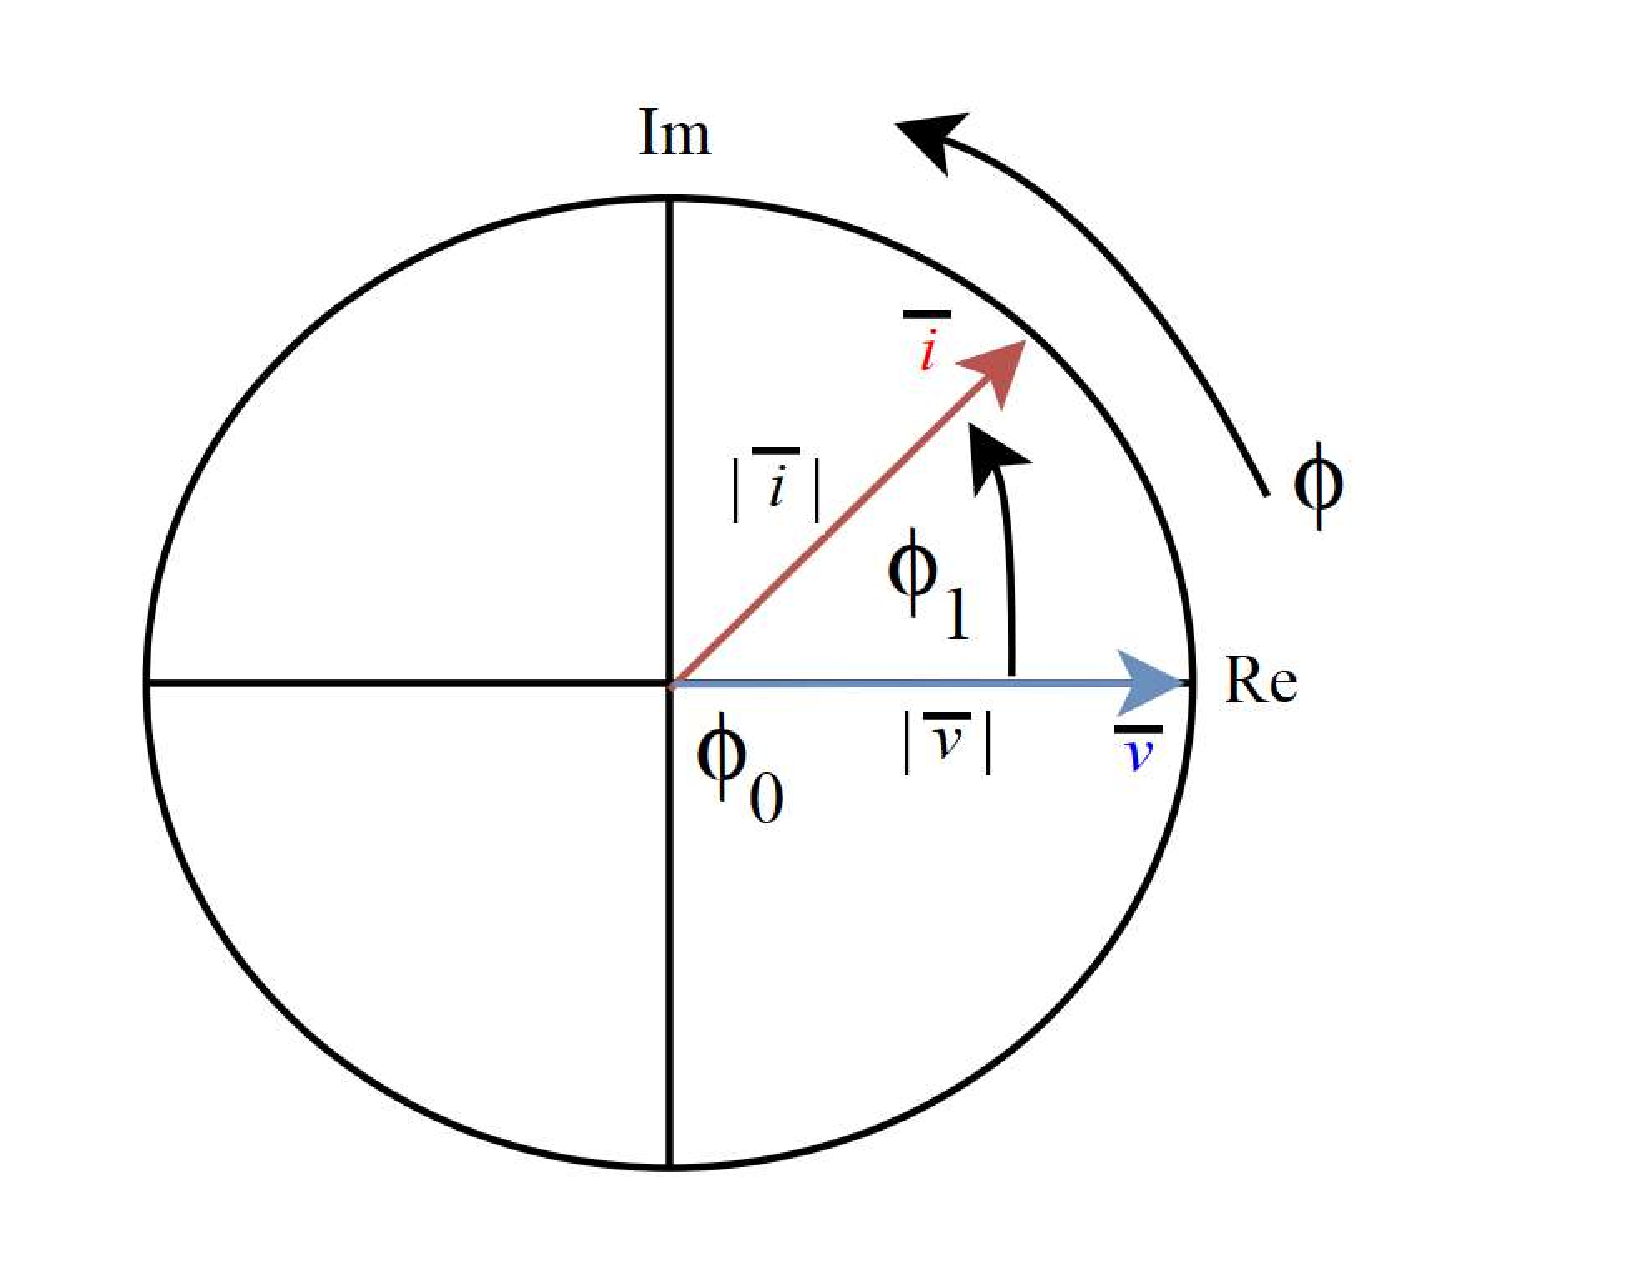
\includegraphics[clip, trim=0 0 0 0, width=0.60\textwidth]{Sections/4_TechnicalAnalysis/Figures/4_1_CapacitancePhasor.pdf}
    \caption{A capacitance causes the current $\bar i$ to lead the voltage $\bar v$. The black $\phi$ arrow signifies the positive direction of the coordinate system.}
    \label{fig:4_1_CapPhasor}
\end{figure}

The voltage vector, $\bar v$, with the phase $\phi_0 = 0$ relative to the real axis, will be the reference for the system because in impedance analyzers the input signal to the DUT will, most often, be a controlled voltage with a known phase and the DUT's phase will be relative to this input waveform. The phase difference $\Delta \phi = \phi_0 - \phi_1$ will correspond to the phase of the $\bar i$ current waveform. The phase of the reference waveform is $\phi_0 = 0$ and this gives the phase of $\bar i$ as shown in eq \ref{eq:4_1_CapPhase}.

\begin{equation}\label{eq:4_1_CapPhase}
    \Delta \phi = \phi_1 - \phi_0=\phi_1 \bigg\rvert_{\phi_0 = 0}
\end{equation}

The impedance of a DUT is the relationship between the voltage and current phasors as shown in equation \ref{eq:4_1_Impedance}.
\begin{equation}\label{eq:4_1_Impedance}
    \bar Z_c = \frac{|\bar v| [cos(\phi_0) +j\cdot sin(\phi_0)]}{|\bar i| [cos(\Delta \phi) +j\cdot sin(\Delta \phi)]}
\end{equation}

Using $\phi_0 = 0$ and $\Delta \phi = \phi_1$ in equation \ref{eq:4_1_Impedance} gets equation \ref{eq:4_1_CapImpedance2}. The numerator reduces to $|\bar v|$ as $cos(0) =1$ and $sin(0) = 0$.
\begin{equation}\label{eq:4_1_CapImpedance2}
    \bar Z_c = \frac{|\bar v|}{|\bar i| [cos(\phi_1) +j\cdot sin(\phi_1)]}
\end{equation}

Applying Eulers formula, and the reciprocal, to eq \ref{eq:4_1_CapImpedance2} gives the final expression for the impedance of a capacitive DUT shown in eq \ref{eq:4_1_CapImpedance4}.
\begin{equation}\label{eq:4_1_CapImpedance4}
    \bar Z_c = \frac{|\bar v|}{|\bar i|} \cdot \mathrm e^{-j\phi_1} = |\bar Z| \cdot \mathrm e^{-j\phi_1} 
\end{equation}
Plotting the impedance vector of a DUT dominated by a capacitance will give a vector pointing into the 4th quadrant as shown in figure \ref{fig:4_1_CapImpedance}.
\begin{figure}[H]
    \centering
    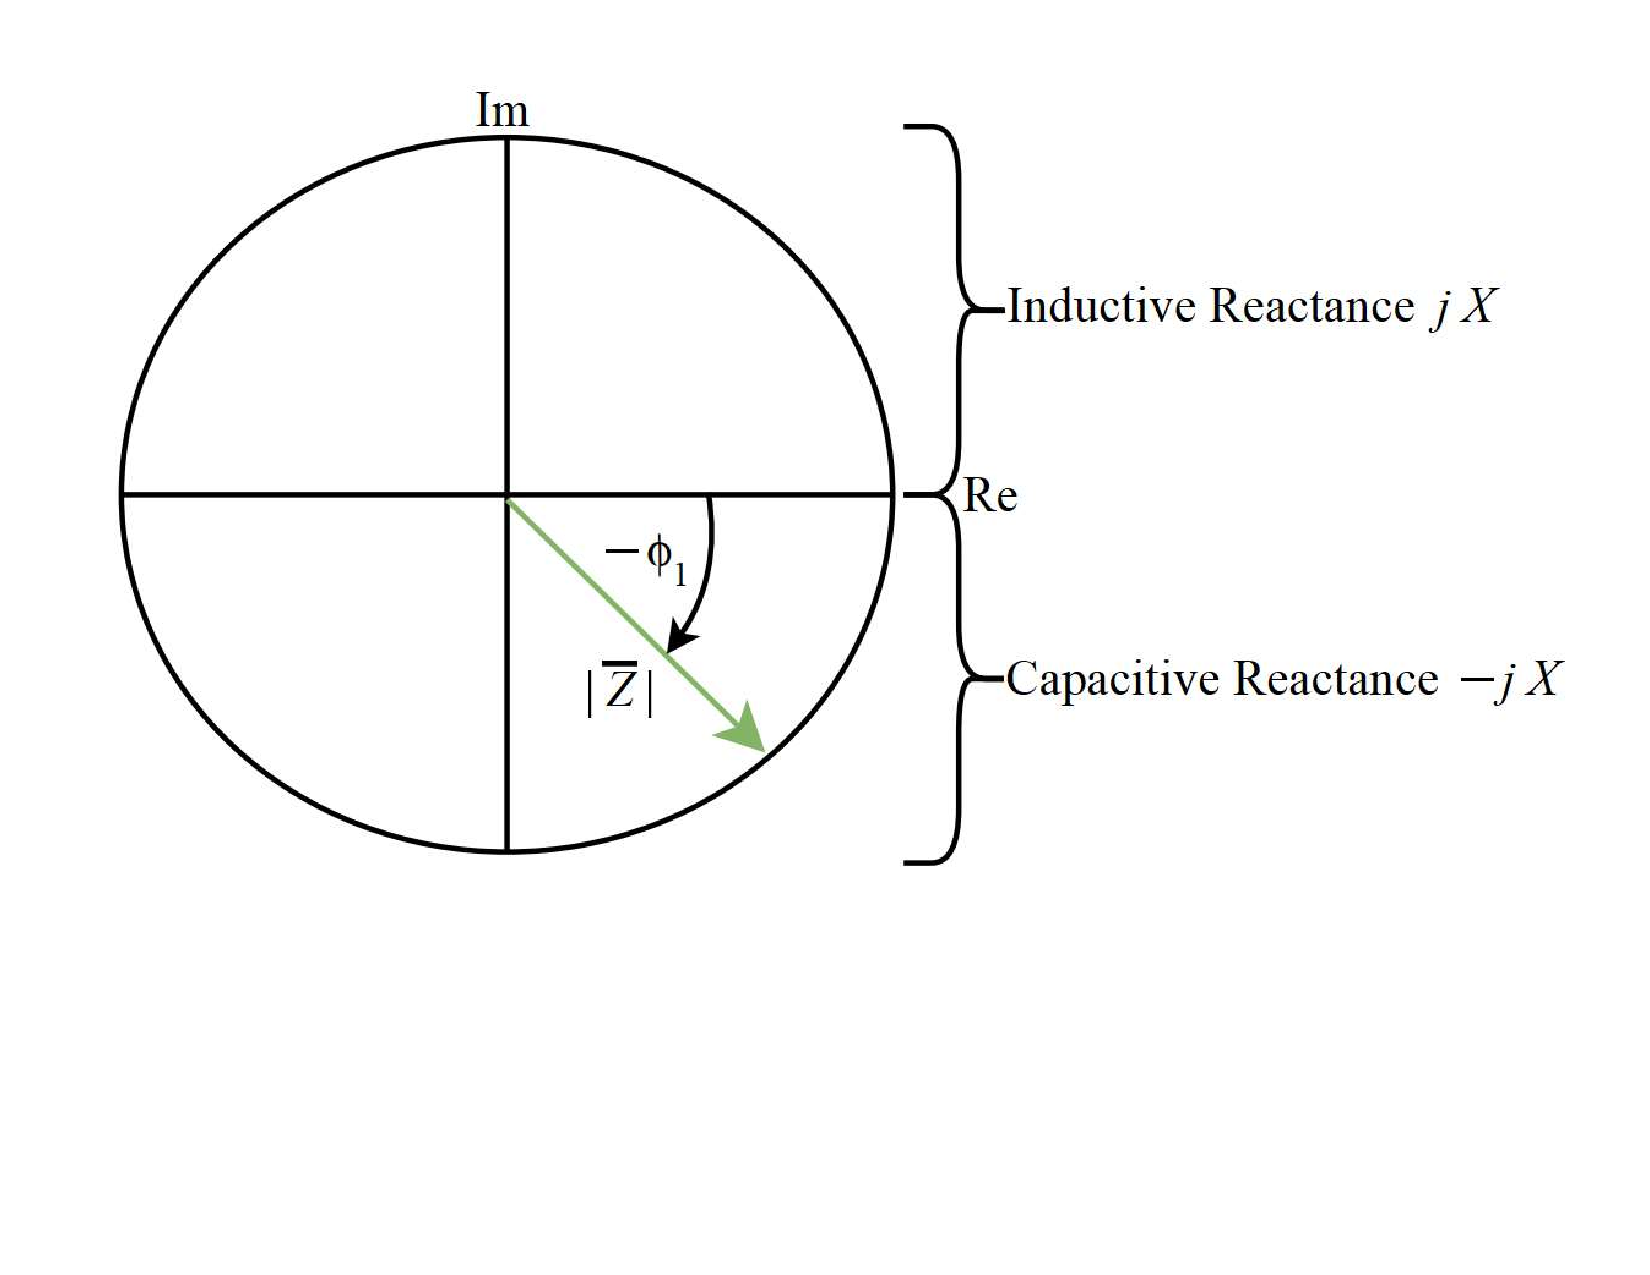
\includegraphics[clip, trim=0 175 0 0, width=0.60\textwidth]{Sections/4_TechnicalAnalysis/Figures/4_1_CapImpedance.pdf}
    \caption{The impedance vector of a capacitive DUT will be located in the 4th quadrant as shown by the $\bar Z$ vector. An impedance pointing into the 4th quadrant is denoted a \textit{capacitive reactance} while an impedance in the 1st quadrant is called a \textit{inductive reactance}.}
    \label{fig:4_1_CapImpedance}
\end{figure}

As shown by figure \ref{fig:4_1_CapImpedance} the sign of the imaginary part of the complex impedance $Z = R \pm jX$ will be an important part to track in order to identify the type of DUT. A similar analysis can be performed with an inductive DUT, in this case the current will lag the voltage as shown on the phasor diagram on figure \ref{fig:4_1_IndPhasor}.
\begin{figure}[H]
    \centering
    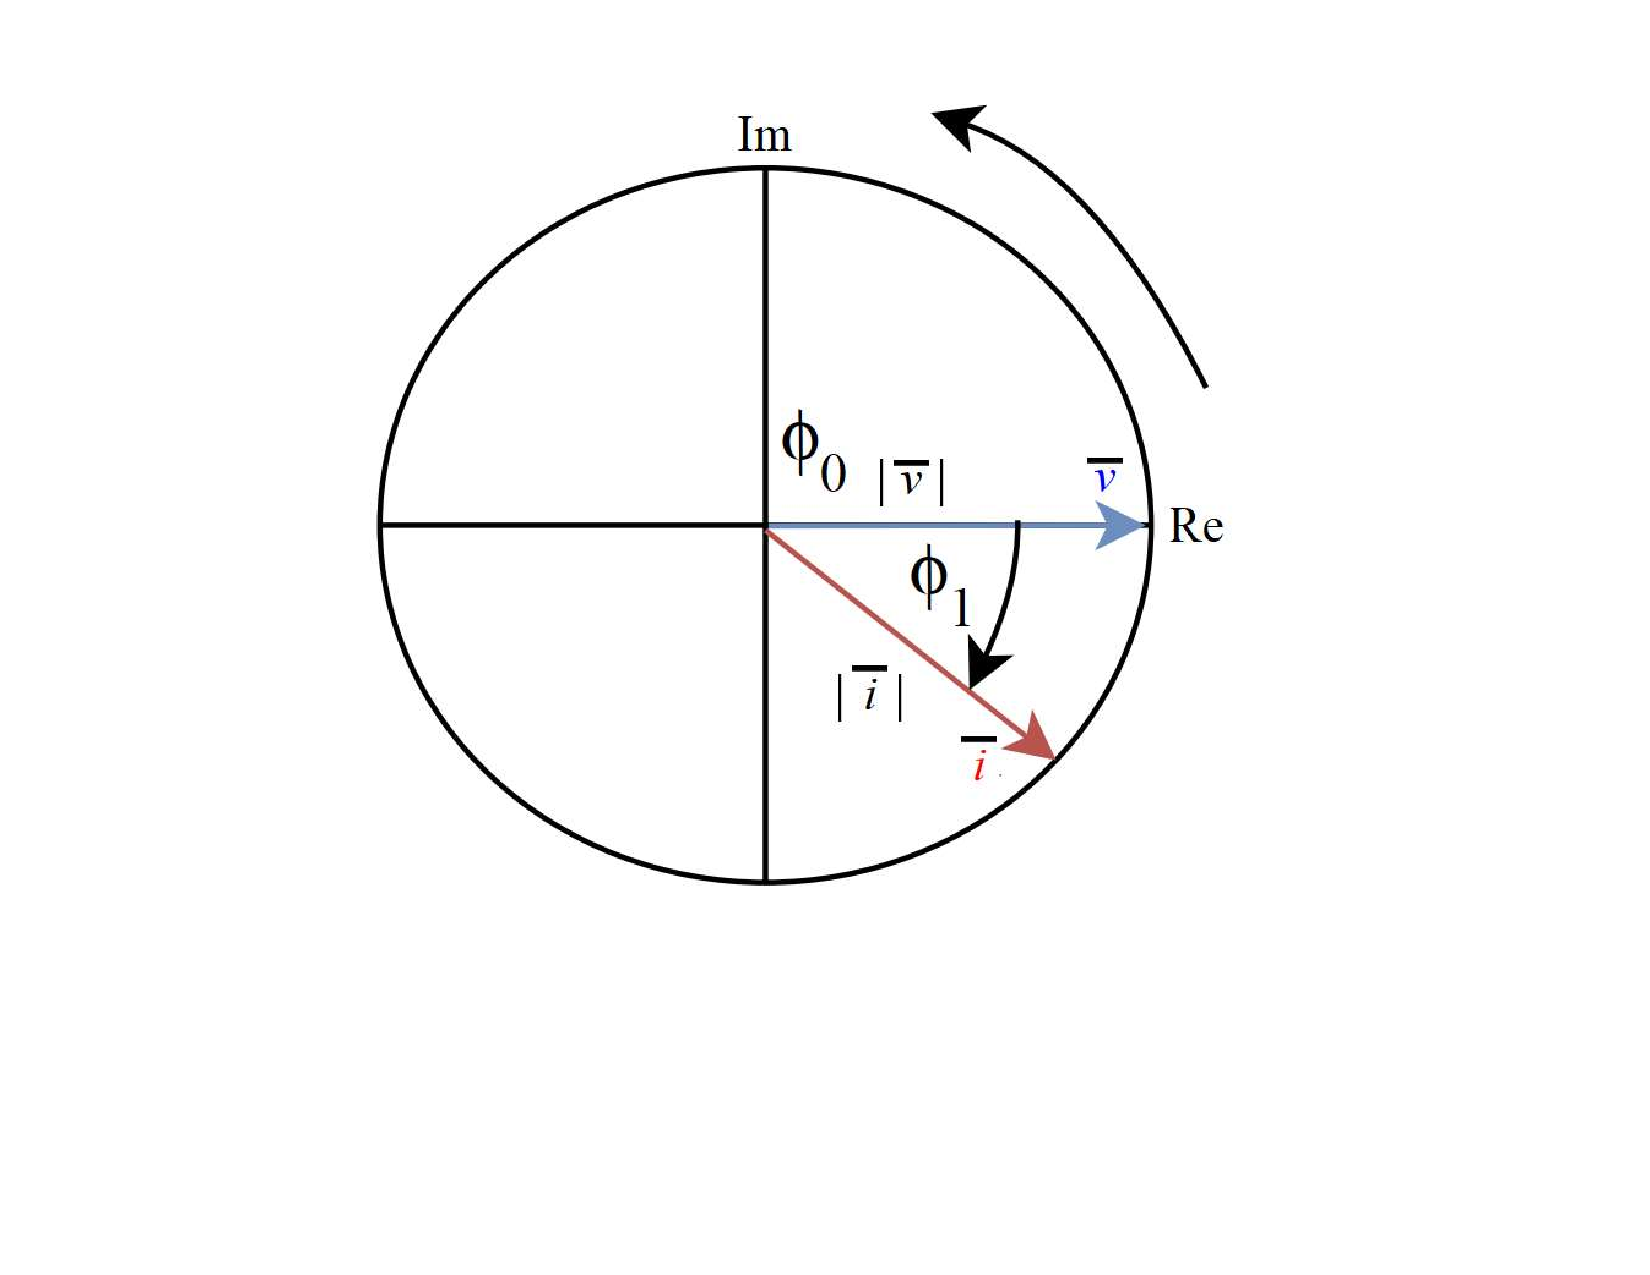
\includegraphics[clip, trim=0 175 0 0, width=0.75\textwidth]{Sections/4_TechnicalAnalysis/Figures/4_1_InductivePhasor.pdf}
    \caption{For an inductive DUT the voltage waveform will lead the current waveform. Note how the phase angle $\phi_1$ of $\bar i$ is going against the established positive direction of the coordinate system.}
    \label{fig:4_1_IndPhasor}
\end{figure}

The current phasor $\bar i$ is lagging the voltage phasor $\bar v$ by a negative phase angle relative to the positive direction of the phasor diagram and will have the phase angle shown in eq \ref{eq:4_1_IndPhase}.

\begin{equation}\label{eq:4_1_IndPhase}
    \Delta \phi = \phi_0 -(-\phi_1) =\phi_1 \bigg\rvert_{\phi_0 = 0}
\end{equation}

Applying eq \ref{eq:4_1_IndPhase} to eq \ref{eq:4_1_Impedance} gives the impedance of an inductive DUT as shown in 
\begin{equation}\label{eq:4_1_IndImpedance2}
    \bar Z_l = \frac{|\bar v|}{|\bar i| [cos(\phi_1) -j\cdot sin(\phi_1)]}
\end{equation}
Once again Eulers formula is applied like in eq \ref{eq:4_1_CapImpedance4} on eq \ref{eq:4_1_IndImpedance2} and gives eq \ref{eq:4_1_IndImpedance3}

\begin{equation}\label{eq:4_1_IndImpedance3} 
    \bar Z_l = \frac{|\bar v|}{|\bar i|} \cdot \frac{1}{cos(\phi_1) - j\cdot sin(\phi_1)} = |\bar Z| \cdot \mathrm (e^{-j\phi})^{-1}
\end{equation}
Eq \ref{eq:4_1_IndImpedance3} is simplified to equation \ref{eq:4_1_IndImpedance4}.
\begin{equation}\label{eq:4_1_IndImpedance4} 
    \bar Z_l =|\bar Z| \cdot \mathrm e^{j\phi}
\end{equation}
Equation \ref{eq:4_1_IndImpedance4} has positive phase and is an impedance vector now pointing into the first quadrant which signifies that it has inductive reactance as shown on figure \ref{fig:4_1_IndImpedance} and figure \ref{fig:4_1_CapImpedance}.

\begin{figure}[H]
    \centering
    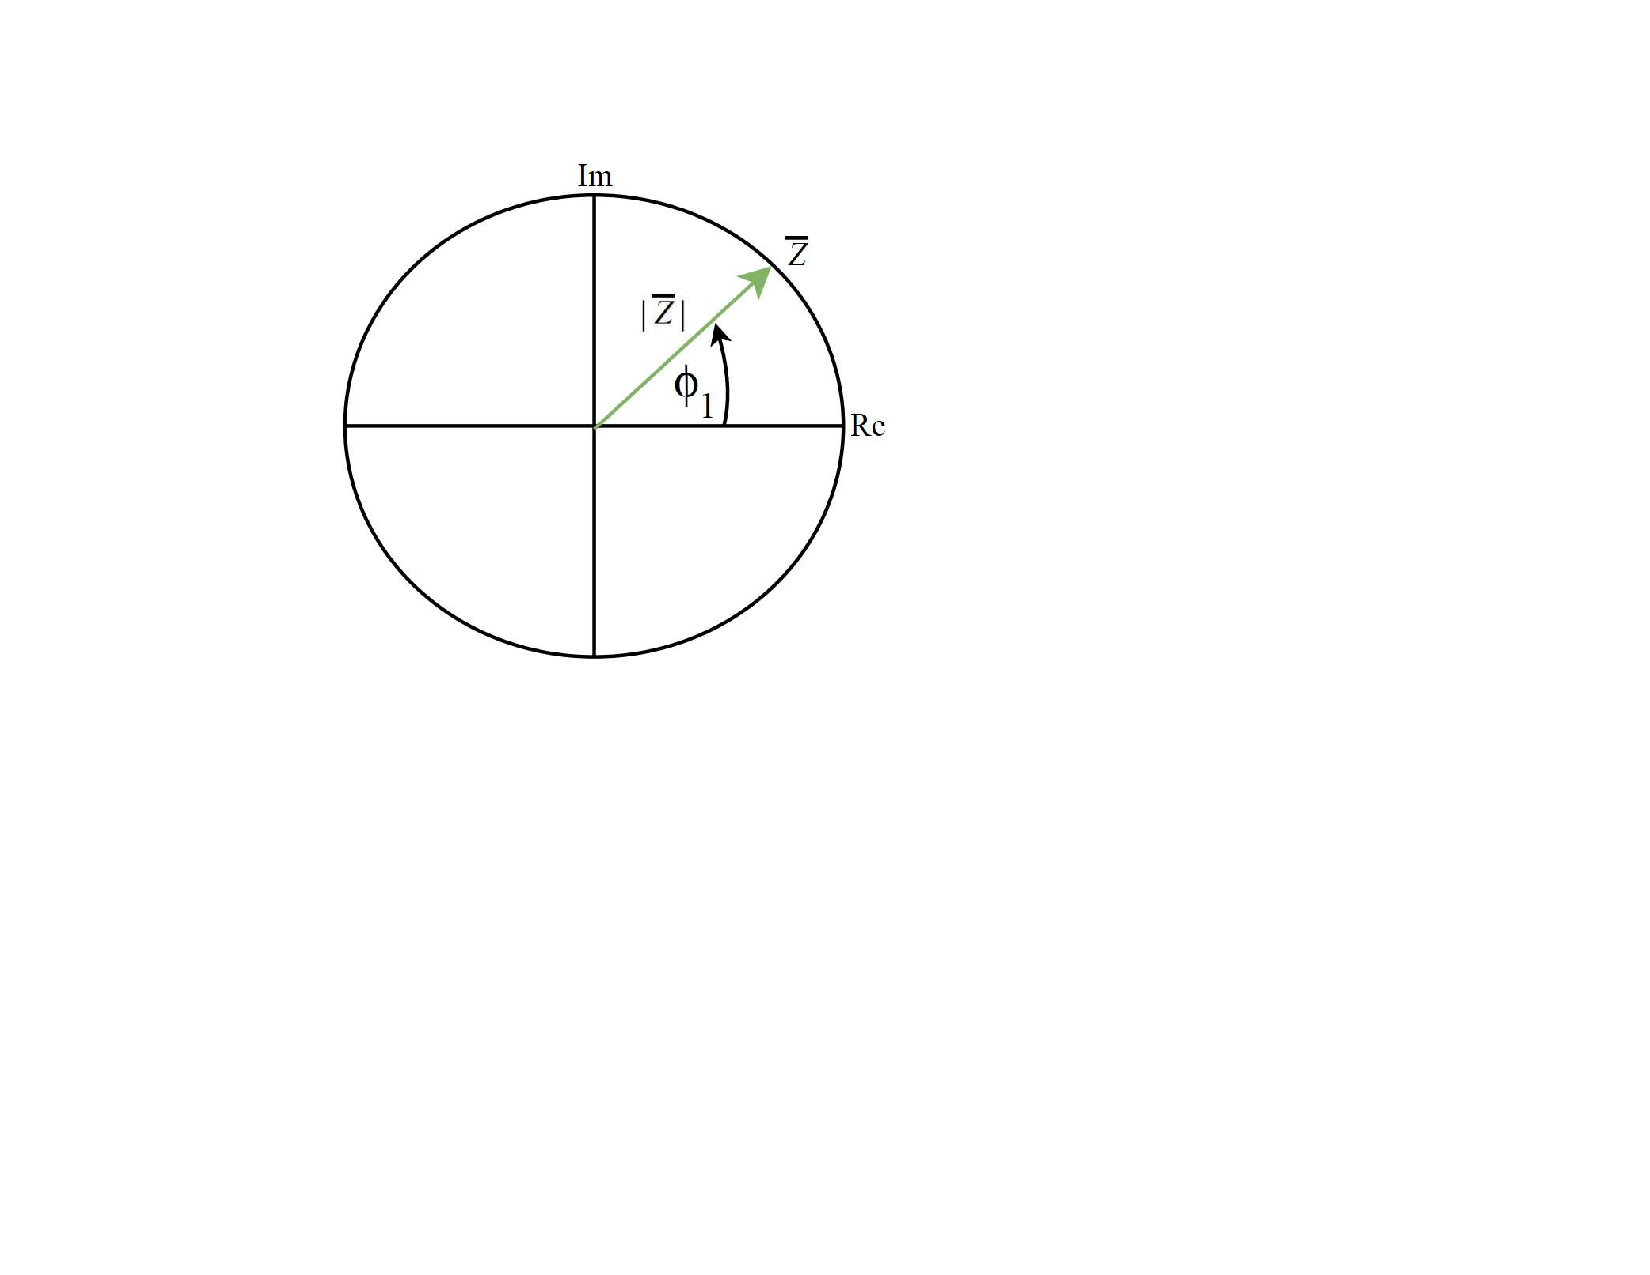
\includegraphics[clip, trim=0 275 0 0, width=1\textwidth]{Sections/4_TechnicalAnalysis/Figures/4_1_IndImpedance.pdf}
    \caption{The impedance an of inductive DUT is pointing into the first quadrant which means the impedance has inductive reactance.}
    \label{fig:4_1_IndImpedance}
\end{figure}

For the case where the DUT has no reactive components the reference voltage waveform will be \textit{in phase} with the resulting current waveform as shown on figure \ref{fig:4_1_ResImpedance}.

\begin{figure}[H]
    \centering
    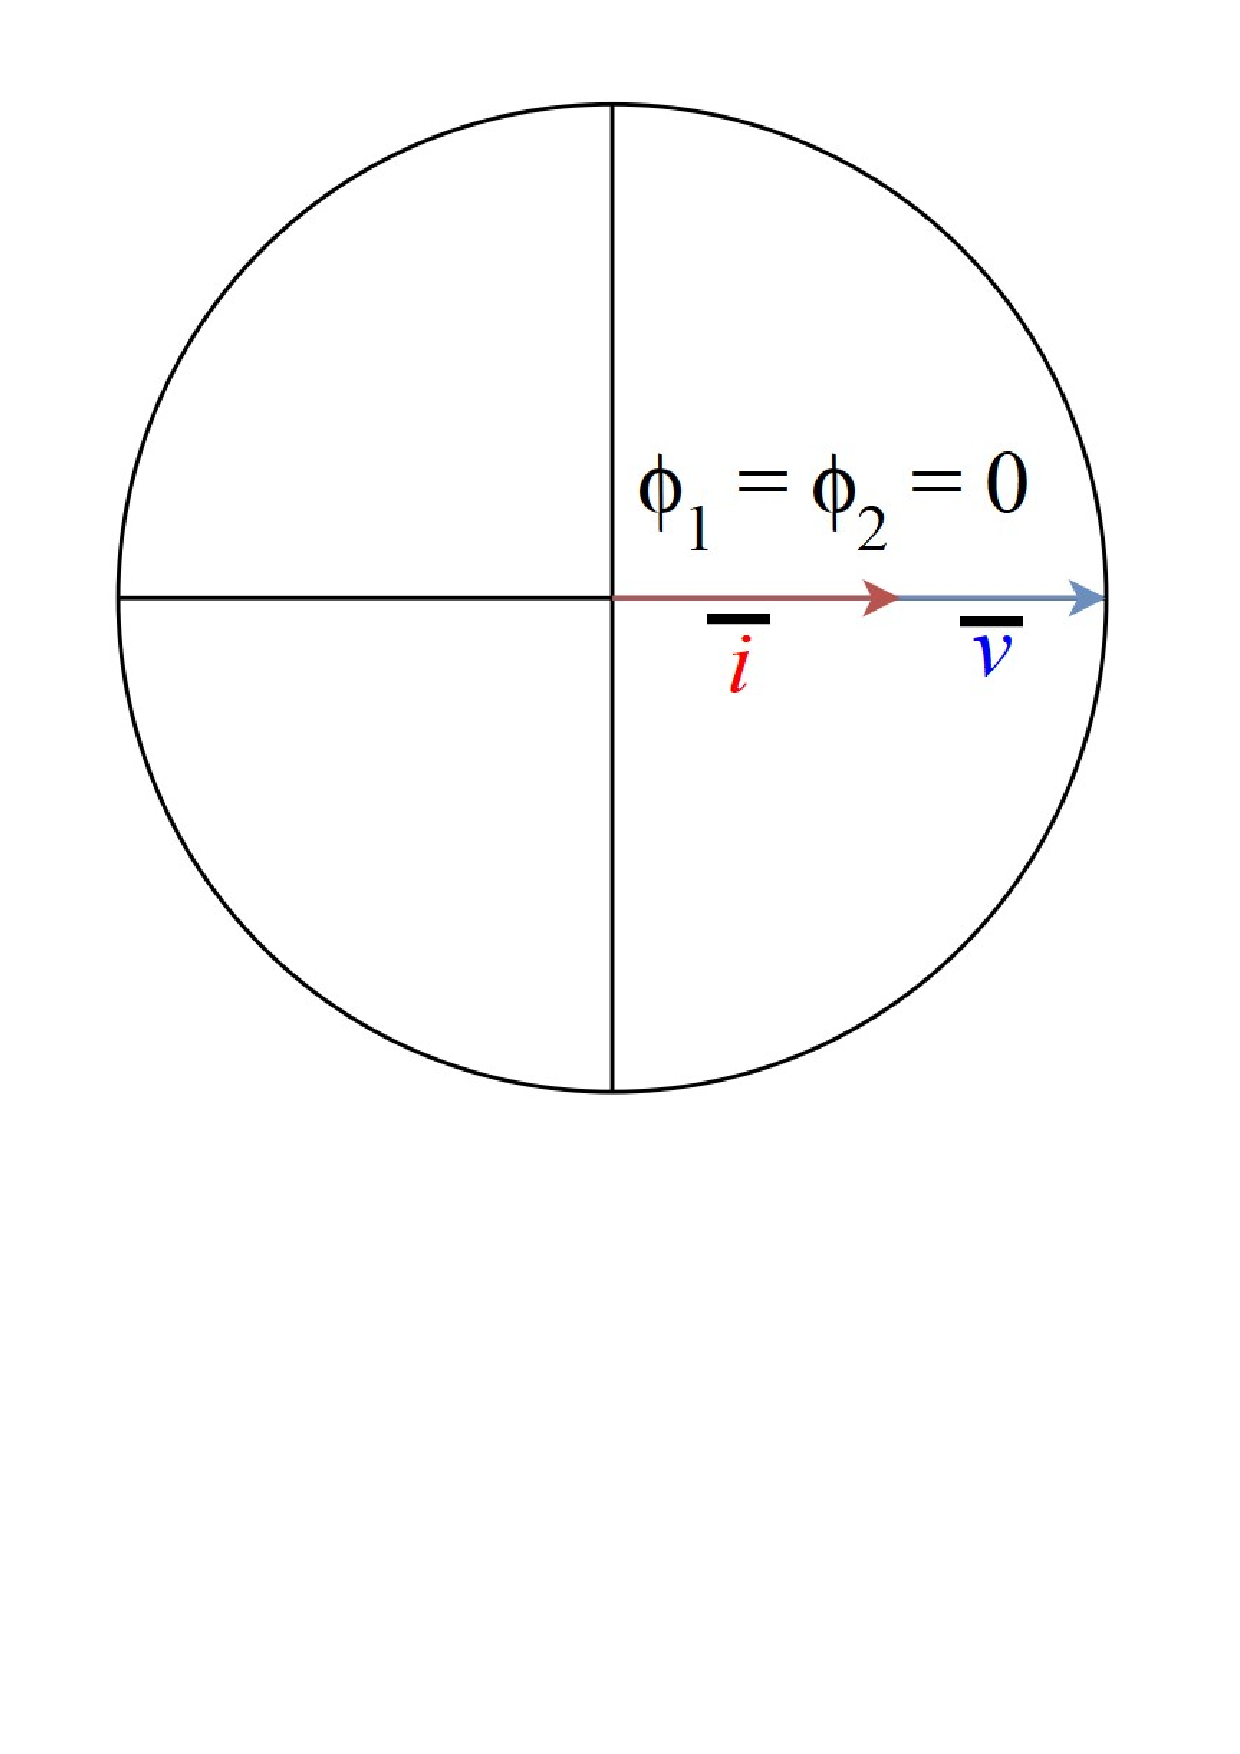
\includegraphics[clip, trim=0 275 0 0, width=0.4\textwidth]{Sections/4_TechnicalAnalysis/Figures/4_1_ResPhasor.pdf}
    \caption{The current vector is in phase with the reference voltage vector. Both vectors lie on the real axis and the impedance will be purely resistive as a result.}
    \label{fig:4_1_ResImpedance}
\end{figure}

The phasor diagram on \ref{fig:4_1_ResImpedance} has the current vector $\bar i$ and the voltage vector $\bar v$ in phase $\phi = 0$ and 
the resulting impedance will be as eq \ref{eq:4_1_Resistance}.
\begin{equation}\label{eq:4_1_Resistance}
    \bar Z_c = \frac{|\bar v| [cos(0) +j\cdot sin(0)]}{|\bar i| [cos(0) +j\cdot sin(0)]}
\end{equation}

With $cos(0) = 1$ and  $sin(0) = 1$ the impedance $\bar Z$ in eq \ref{eq:4_1_Resistance} is purely resistive. It has no imaginary component and thus has no phase shift and depends only on the magnitude of $\bar i$ and $\bar v$ as shown in eq \ref{eq:4_2_Resistance}
\begin{equation}\label{eq:4_2_Resistance}
    \bar Z_c = \frac{|\bar v|}{|\bar i|}
\end{equation}

Equations \ref{eq:4_1_CapImpedance4}, \ref{eq:4_1_IndImpedance4} and \ref{eq:4_2_Resistance} show that, in order to calculate the impedance of a DUT, an impedance analyzer must be able to measure the magnitude and phase of the reference voltage waveform $\bar v_{ref}$ along with the magnitude and phase of the resulting current waveform $\bar i_{dut}$. The system may already have some information on $\bar v_{ref}$ but in either case it must be known. It is possible to calculate the value of $L, C, R, D, Q..$ and so on once the impedance is known as will be shown in the next chapter.
\section{Typical Impedance Measurement Principles} \label{sec:TypicalMeasPrin}

\subsection{Wheatstone Bridge} \label{ssec:BridgeCircuits}
The Wheatstone bridge has been around since the 1800 hundreds, and was among the very first methods used to characterize an unknown impedance. Originally only used for DC resistance measurements, but with a few modifications it was expanded to characterize impedances as well. 
The circuit can be seen in figure \ref{fig_4_2_WheatstoneBridge}, where $Z_1$ is the unknown device,
 often referred to as the DUT.
 
A null detector is present across the two nodes, this allows the two impedance ratios $Z_1/Z_3$ and $Z_2/Z_4$
to be matched. If there is \SI{0}{\volt} at all times across node b and d, then the ratio of $Z_1/Z_3$ will match that of
 $Z_2/Z_4$, and the
phase angle will be given as $\theta_1 - \theta_2 = \theta_2 - \theta_4$. 

\begin{figure}[H]
    \centering
    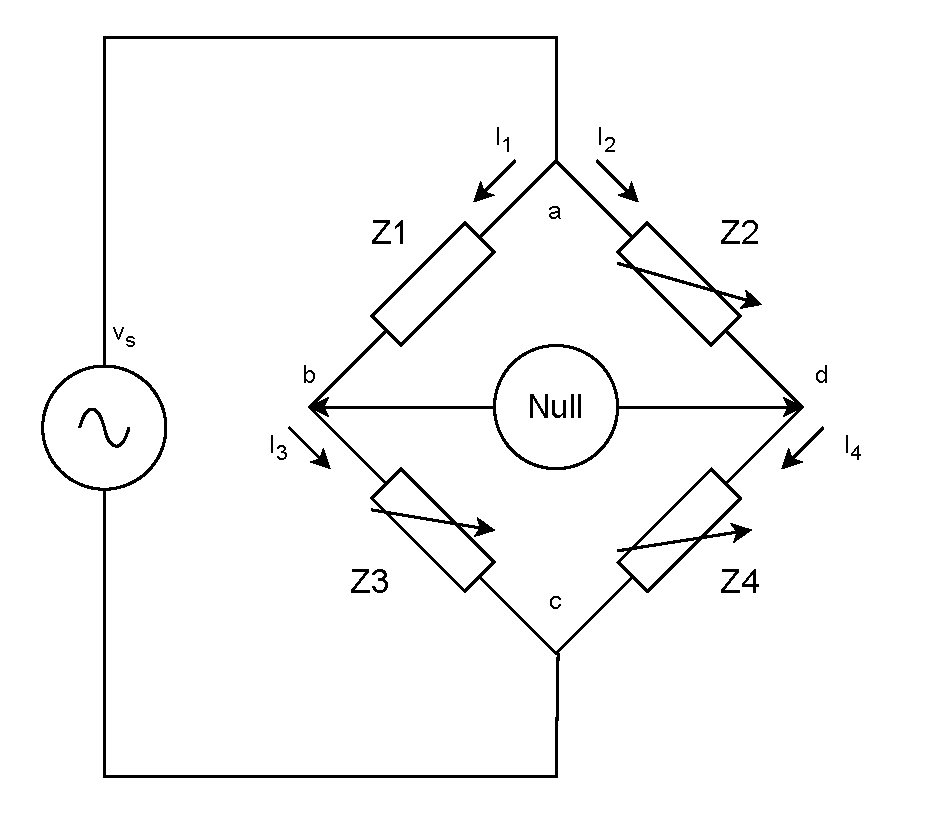
\includegraphics[width=0.75\textwidth]{Sections/4_TechnicalAnalysis/Figures_JFT/WheatstoneBridgeAC.pdf}
    \caption{A typical AC Wheatstone bridge, where Z1 is the device under test.}
    \label{fig_4_2_WheatstoneBridge}
\end{figure}

The relationship between the different impedances can be described by analyzing the bridge. The voltage across $Z_1$ and $Z_2$ can
be described as in equation \ref*{eq:4_2_TopWheatstone}.

\begin{equation}
    \begin{split}
        \label{eq:4_2_TopWheatstone}
        i_1 &= \frac{v_s-v_1}{Z_1} \Rightarrow -i_1 Z_1 +v_s = v_1 \\
        i_2 &= \frac{v_s-v_1}{Z_2} \Rightarrow -i_2 Z_2 + v_s = v_2
    \end{split}
\end{equation}

Under the assumption that the null detector reads zero, and the same voltage is present at node b and d, then the voltage
across $Z_1$ must be equal to that across $Z_2$. From this equation \ref{eq:4_2_TopWheatStone2} can be constructed, showing the
relationship between currents and impedances for the top most resistors of the bridge.

\begin{equation}
    \begin{split}
        \label{eq:4_2_TopWheatStone2}
        v_1 &= v_2 \Rightarrow -i_1 Z_1 +v_s = -i_2 Z_2 + v_s \\
        i_1 Z_1 &= i_2 Z_2 \Rightarrow \frac{i_2}{i_1} = \frac{Z_1}{Z_2}
    \end{split}
\end{equation}

In much the same way, the lower half of the bridge can be described as seen in equation \ref{eq:4_2_BotWheatstone}

\begin{equation}
    \label{eq:4_2_BotWheatstone}
    \frac{i_4}{i_3} = \frac{Z_3}{Z_4}
\end{equation}

A proper null detector will not interfere with the circuit it is measuring, so no current should flow in to or out of the
null detector, meaning that $i_1$ must equal $i_3$ and $i_2 = i_4$, as the components are in series. Under this assumption, it can be
shown that the unknown impedance $Z_1$ and its phase angle can be found from the 3 other know impedances and phase angles, as shown
in equation \ref{eq:4_2_MatchedWheatstone}.

\begin{equation}
    \begin{split}
        \label{eq:4_2_MatchedWheatstone}
        \frac{i_2}{i_1} &= \frac{i_4}{i_3} \Rightarrow \frac{Z_1}{Z_2} = \frac{Z_3}{Z_4} \Rightarrow \frac{Z_1}{Z_3} = \frac{Z_2}{Z_4} \\
        \frac{|Z_1|\e^{j\theta_1}}{|Z_3|\e^{j\theta_3}} &= \frac{|Z_2|\e^{j\theta_2}}{|Z_4|\e^{j\theta_4}}
        \Rightarrow \frac{|Z_1|}{|Z_3|}\e^{j\left(\theta_1-\theta_3\right)} = \frac{|Z_2|}{|Z_4|}\e^{j\left(\theta_2-\theta_4\right)} \\
        \\
        \Rightarrow \frac{|Z_1|}{|Z_3|} &= \frac{|Z_2|}{|Z_4|} \quad and \quad \theta_1-\theta_3 = \theta_2-\theta_4 \\
        \Rightarrow |Z_1| &= \frac{|Z_2|\cdot|Z_3|}{|Z_4|} \quad and \quad \theta_1 = \theta_2+\theta_3-\theta_4
    \end{split}
\end{equation}

The AC Wheatstone bridge has proven itself to be highly accurate, but is somewhat frequency limited, and expensive, as it requires a
vast arsenal of stable and well known capacitors and resistors to be used for the 3 adjustable impedances. This is something that
is typically found in a metrology grade laboratory and not in an instrument.


\subsection{I-V Method} \label{ssec:IVMethod}
The I-V method or current voltage method, has already been shortly introduced in section \ref{sec:MeasureReactiveComponents}, here it was realized by the use of a function generator and an oscilloscope. In this chapter, the I-V method will however be introduced in a more broad spectrum, that is to say, the general principle of the method will be outlined.

In general, two principles of the I-V method are implemented in the industry, either the I-V method or the RF I-V method. The I-V method offers good accuracy 
and a broad bandwidth, from a few hertz to about \SIQ{100}{\mega\hertz}. The RF I-V method uses RF principles such as directional couplers and extends the bandwidth up to about \SIQ{3}{\giga\hertz}, it is however not suitable for frequencies below the mega hertz region\cite{Keysight_Impedance}. This chapter will solely focus on the I-V method as the RF frequency range is not of interest to this project.

The principle of the I-V method is simple; measure current and voltage, and determine the angle between them. This can be implemented in numerous different ways, using coupled inductors to measure the current, or a series shunt where the voltage-drop can be measured across, to name a few. 

\begin{figure}[H]
    \centering
    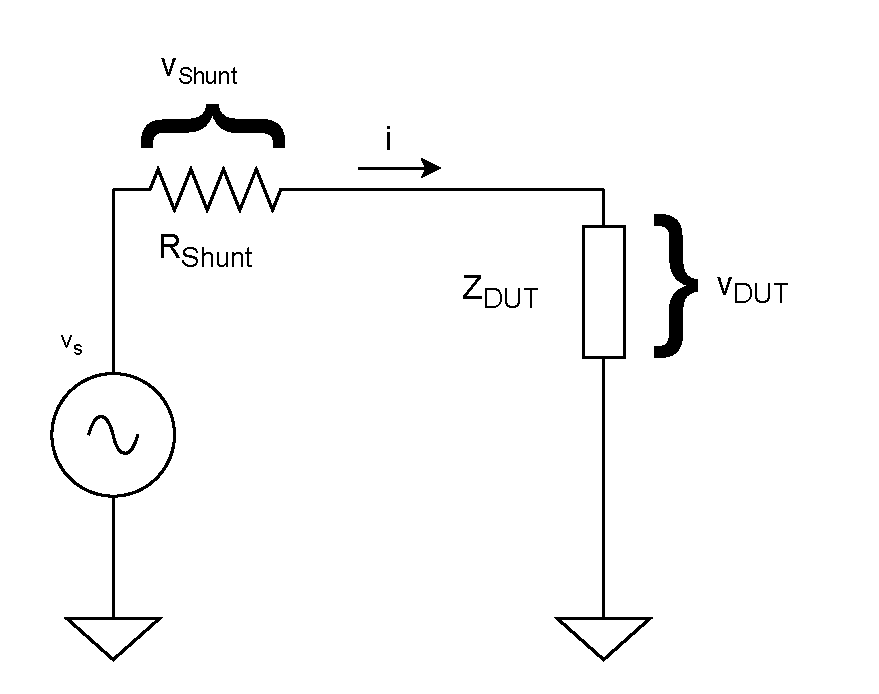
\includegraphics[width=0.75\textwidth]{Sections/4_TechnicalAnalysis/Figures_JFT/IV_Method.pdf}
    \caption{The I-V Method implemented with a current shunt to measure the current}
    \label{fig_4_2_IVMethod}
\end{figure}

The principle of the I-V method can be seen in figure \refq{fig_4_2_IVMethod}. The current in the system can be described by an amplitude and phase, as can the voltage, as seen in equation \ref{eq:4_2_2_IVVectors}, where $v$ is the voltage across the DUT and $i$ is the current through it. It is assumed that the current is the same through the shunt and the DUT.

\begin{equation}
    \label{eq:4_2_2_IVVectors}
    \begin{split}
        \bar{i} & = |i|\cdot\e ^{j\theta_i} \Rightarrow \bar{i} = \frac{|v_{shunt}|}{R_{shunt}}\e ^{j\theta_{v\:shunt}}\\
        \bar{v_{DUT}} & = |\bar{v_{DUT}}| \cdot\e ^{j\theta_{v\:DUT}}
    \end{split}
\end{equation}

The impedance can then be calculated from the two voltages of the system, i.e. the shunt voltage and the DUT voltage, as seen in equation \ref{eq:4_2_2_Impedance}.

\begin{equation}
    \label{eq:4_2_2_Impedance}
    \begin{split}
        Z & = \frac{v_{DUT}}{i} \Rightarrow \bar{Z} = \frac{|v_{DUT}| \cdot\e ^{j\theta_{v\:DUT}}}{\frac{|v_{shunt}|}{R_{shunt}}\e ^{j\theta_{v\:shunt}}} \\
        \bar{Z} & = \frac{|v_{DUT}|\cdot R_{shunt}}{|v_{shunt}|}\cdot \e ^{j\left(\theta_{v\:DUT}-\theta_{v\:shunt}\right)}
    \end{split}
\end{equation}

This is the I-V method in its simplest form. The shunt used is however required to be swapped depending on the DUT, as a small shunt would be poorly suited to measure small currents. In practice, compensation elements can also be required to ensure stability, as some systems can become unstable under large capacitive loads.


%Bibliography
\printbibliography[heading = bibintoc]

%Appendix
\appendix

\chapter{GIThub} \label{App:GIThub}

ref til git






\end{document}
